%\documentclass[a4paper,10pt]{article}
\documentclass[12pt]{article}
\usepackage{graphicx}
\usepackage{amssymb}
\usepackage{amsmath}
\usepackage{longtable}
\usepackage{wrapfig}
%\usepackage{color}
%\usepackage{amsthm}
\usepackage[utf8]{inputenc}
\usepackage[T1]{fontenc}
\usepackage{lmodern}
\usepackage{listings}
\usepackage[usenames,dvipsnames]{color}
\usepackage{fancyhdr}
\usepackage{fullpage}
%\usepackage[top=tlength, bottom=blength, left=llength, right=rlength]{geometry}
%\usepackage{geometry}
%\usepackage[a4paper]{geometry}
\definecolor{MyDarkGreen}{rgb}{0.0,0.4,0.0}
%\usepackage[pdftex]{graphicx}
%\usepackage{mathtools}
\usepackage{listings}
\lstset{language=C++}
%===========================================================================================
% Numbering Equations
%\numberwithin{equation}{section} %sets equation numbers <chapter>.<section>.<index>
\numberwithin{equation}{subsection} %sets equation numbers <chapter>.<section>.<subsection>.<index>
%\numberwithin{equation}{subsubsection} %sets equation numbers <chapter>.<section>.<subsection>.<subsubsection>.<index>


%===================================================================================================================
% Basic Commands for Page settings,Chapters, Appendices, Sections, etc..
%====================================================================================================================
%\setlength{\oddsidemargin}{.5in} \setlength{\topmargin}{0in}
%\setlength{\headheight}{.2in} \setlength{\headsep}{.2in}
%\setlength{\textwidth = 6.0in} \setlength{\textheight = 8.3in}

\setlength{\oddsidemargin}{0.6in} \setlength{\topmargin}{-0.3in} %adjust side margins and top margins
\setlength{\headheight}{.2in} \setlength{\headsep}{.2in}
\setlength{\textwidth = 6.0in} \setlength{\textheight = 8.3in}



\def\thebiblio#1{\list
{[\arabic{enumi}]}{\settowidth\labelwidth{[#1]}\leftmargin\labelwidth
\advance\leftmargin\labelsep
\usecounter{enumi}}
\def\newblock{\hskip .11em plus .33em minus .07em}
\sloppy\clubpenalty4000\widowpenalty4000
\sfcode`\.=1000\relax}
\let\endthebiblio=\endlist

\newcommand{\sect}[1]{% Basic settings for general chapters
\cleardoublepage
\clearpage
\newpage
\begin{center}
\addtocounter{section} {1}
\setcounter{subsection} {0}
\section* {\normalsize \bf{CHAPTER \thesection \\ #1}}
\addcontentsline{toc}{section}{CHAPTER
\protect\numberline{\thesection : } #1\dotfill}
\end{center}
\thispagestyle{myheadings} }

\newcommand{\appen}[1]{% Basic settings for appendix chapters
\cleardoublepage
\clearpage
\newpage
\begin{center}
\addtocounter{section} {1}
\renewcommand{\thesection}{\Alph{section}}
\setcounter{subsection} {0}
\setcounter{table}{0}
\section* {\normalsize \bf{APPENDIX \thesection \\ #1}}
\addcontentsline{toc}{section}{APPENDIX
\protect\numberline{\thesection : } #1\dotfill}
\end{center}
\renewcommand{\thesubsection}{\Alph{section}.\arabic{subsection}}
\renewcommand{\thesubsubsection}{\Alph{section}.\arabic{subsection}.\arabic{subsubsection}}
\renewcommand{\theequation}{\Alph{section}.\arabic{equation}}
\renewcommand{\thetable}{\Alph{section}.\arabic{table}}

\thispagestyle{myheadings} }

%===================================================================================================================
% Basic Commands for Theorem, Lemma,Proposition,etc.....

\renewcommand{\baselinestretch}{2}
\renewcommand{\arraystretch}{.5}
\newcommand{\qed}{\hfill$\Box$}
\newtheorem{fact}{Theorem}[section]
\newtheorem{claim}{Claim}
\newtheorem{theorem}[fact]{Theorem}
\newtheorem{word}[fact]{Definition}
\newtheorem{prop}[fact]{Proposition}
\newtheorem{ob}[fact]{Observation}
\newtheorem{Corollary}[fact]{Corollary}
\newtheorem{corollary}[fact]{Corollary}
\newtheorem{lemma}[fact]{Lemma}
\newtheorem{Guess}[fact]{Conjecture}
\newtheorem{conj}[fact]{Conjecture}
\def\theotheorem{A\arabic{theorem}}
\newtheorem{mydef}{Definition}
%\newtheorem{theorem}{Theorem}[section]
%\newtheorem{lemma}[theorem]{Lemma}
%\newtheorem{proposition}[theorem]{Proposition}
\newtheorem{thm}{Theorem}
\newtheorem{lem}{Lemma}[thm]
%\newtheorem{corollary}[theorem]{Corollary}
%\newtheorem{cor}[theorem]{Corollary}
\newenvironment{proof}[1][Proof]{\begin{trivlist}
\item[\hskip \labelsep {\bfseries #1}]}{\end{trivlist}}
\newenvironment{definition}[1][Definition]{\begin{trivlist}
\item[\hskip \labelsep {\bfseries #1}]}{\end{trivlist}}
\newenvironment{example}[1][Example]{\begin{trivlist}
\item[\hskip \labelsep {\bfseries #1}]}{\end{trivlist}}
\newenvironment{remark}[1][Remark]{\begin{trivlist}
\item[\hskip \labelsep {\bfseries #1}]}{\end{trivlist}}
%================================================================================
%%%%%%%%%%%commands for problem
%================================================================================
\makeatletter
\newenvironment{problem}{\@startsection
       {section}
       {1}
       {-.2em}
       {-3.5ex plus -1ex minus -.2ex}
       {2.3ex plus .2ex}
       {\pagebreak[3]%forces pagebreak when space is small; use \eject for better results
       \large\bf\noindent{Problem }
       }
       }
       {%\vspace{1ex}\begin{center} \rule{0.3\linewidth}{.3pt}\end{center}}
       \begin{center}\large\bf \ldots\ldots\ldots\end{center}}
\makeatother


%
%Fancy-header package to modify header/page numbering
\pagestyle{fancy}
%\addtolength{\headwidth}{\marginparsep} %these change header-rule width
%\addtolength{\headwidth}{\marginparwidth}
\lhead{Problem \thesection} \chead{} \rhead{\thepage}
\lfoot{\small\scshape course name} \cfoot{} \rfoot{\footnotesize
PS\#}
\renewcommand{\headrulewidth}{0.3pt}
\renewcommand{\footrulewidth}{.3pt}
%\setlength\voffset{-0.25in} \setlength\textheight{648pt} \maketitle
%\maketitle
 %\thispagestyle{empty}



%===========================================================================
% commands for displaying codes in appendix
%============================================================================

	
	%===========================================================================
	% commands for displaying codes in appendix
	%============================================================================
	\usepackage{listings}
	%===========================================================================
	% commands for displaying codes in appendix
	%============================================================================
	\lstloadlanguages{r}%
	\lstset{language=r }
	
	% Includes an r script.
	% The first parameter is the label, which also is the name of the script
	%   without the .m.
	% The second parameter is the optional caption.
	\definecolor{codegreen}{rgb}{0,0.6,0}
	\definecolor{codegray}{rgb}{0.5,0.5,0.5}
	\definecolor{codepurple}{rgb}{0.58,0,0.82}
	\definecolor{backcolour}{rgb}{0.95,0.95,0.92}
	
	\lstdefinestyle{mystyle}{
		backgroundcolor=\color{white},   
		commentstyle=\color{codegreen},
		keywordstyle=\color{magenta},
		numberstyle=\tiny\color{codegray},
		stringstyle=\color{codepurple},
		basicstyle=\footnotesize,
		breakatwhitespace=false,         
		breaklines=true,                 
		captionpos=b,                    
		keepspaces=true,                 
		numbers=left,                    
		numbersep=5pt,                  
		showspaces=false,                
		showstringspaces=false,
		showtabs=false,                  
		tabsize=2
	}
	
	\lstset{style=mystyle}
	



\begin{document}
\pagestyle{empty}
\pagenumbering{roman}

%================================================ Approval Page ===================================================
\newpage
%\nocounter
 \pagestyle{plain}
 \thispagestyle{empty}% takes out page numbering

\begin{center}

{\bf APPROVAL} \\ [.05in]
{\bf This is to certify that the Graduate Committee of }\\
Nana  Akwasi Abayie Boateng \\ [-.1in] met on the \\ [-.1in] 14th \
day of \ June, 2012.
\\ [.25in]
\end{center}

\baselineskip=20 pt

 The committee read and examined his/her thesis,
supervised his/her defense of it in an oral examination, and decided
to recommend that his/her study should be submitted to the Graduate
Council, in partial fulfillment of the requirements for the  degree
of Master of Science in Mathematics.

\vspace{.3in}

\noindent
\makebox[3.4in][l]{}\makebox[2.0in][l]{\rule{2.5in}{.01in}}\\[-.1in]
\makebox[3.4in][l]{} \makebox[2.0in][l]{\it Dr. A.Q.M.Khaliq}\\[-.1in]
\makebox[3.4in][l]{} \makebox[2.0in][l]{Chair, Graduate Committee } \\[.1in]
\makebox[3.4in][l]{} \makebox[2.0in][l]{\rule{2.5in}{.01in}} \\[-.1in]
\makebox[3.4in][l]{} \makebox[2.0in][l]{\it Dr. Zachariah Sinkala} \\[.1in]
\makebox[3.4in][l]{} \makebox[2.0in][l]{\rule{2.5in}{.01in}} \\[-.1in]
\makebox[3.4in][l]{} \makebox[2.0in][l]{\it Dr. Yuri Melnikov} \\[.1in]
\makebox[3.4in][l]{} \makebox[2.0in][l]{\rule{2.5in}{.01in}} \\[-.1in]
\makebox[3.4in][l]{} \makebox[2.0in][l]{\it Dr. James Hart} \\[-.1in]
\makebox[3.4in][l]{}\makebox[2.0in][l]{ Graduate Coordinator,} \\[-.1in]
\makebox[3.4in][l]{}\makebox[2.0in][l]{ Department of Mathematical Sciences} \\[.1in]
\makebox[3.4in][l]{} \makebox[2.0in][l]{\rule{2.5in}{.01in}} \\[-.1in]
%\makebox[3.4in][l]{} \makebox[2.0in][l]{\it Dr. Don Nelson} \\[-.1in]
%\makebox[3.4in][l]{}\makebox[2.0in][l]{ Chair,} \\[-.1in]
%\makebox[3.4in][l]{}\makebox[2.0in][l]{ Department of Mathematical Sciences} \\[.1in]
%\makebox[3.4in][l]{Signed on behalf of } \makebox[2.0in][l] {\rule{2.5in}{.01in}}\\[-.1in]
\makebox[3.4in][l]{the Graduate Council}\makebox[2.0in][l]{\it Dr. Michael Allen} \\[-.1in]
\makebox[3.4in][l]{}\makebox[2.0in][l]{ Dean,} \\[-.1in]
\makebox[3.4in][l]{}\makebox[2.0in][l]{ School of Graduate Studies}
\newpage
%================================================ Title Page ======================================================
\begin{center}
\thispagestyle{empty} % takes out page numbering
  {MESHFREE METHODS FOR THE THE BLACK-SCHOLES  PARTIAL DIFFERENTIAL EQUATION \\ [.07in]} \rm
\rule{1.25in}{.01in}\\[.0 in]

\vspace{.6in}

A Thesis \\ [.06  in]
Presented to the Faculty of the  Department of Mathematical Sciences \\[.06in]
Middle Tennessee State University \\ [.06in]
\rule{1.25in}{.01in}\\

\vspace{.6in}

In Partial Fulfillment \\[.06 in]
of the Requirements for the Degree \\ [.06 in]
Master of Science in Mathematical Sciences \\ [.06 in]
\rule{1.25in}{.01in}\\

\vspace{.6in}

by  \\ [.06in]
{Nana  Akwasi Abayie Boateng} \\[.06in]
{August 2012}
\end{center}

%%================================================ Approval Page ===================================================
%\newpage
%
%\pagestyle{plain}
%
%\begin{center}
%
%{\bf APPROVAL} \\ [.05in]
%{\bf This is to certify that the Graduate Committee of }\\
%Nana  Akwasi Abayie Boateng \\ [-.1in] met on the \\ [-.1in] 14th \
%day of \ June, 2012.
%\\ [.25in]
%\end{center}
%
%\baselineskip=20 pt
%
% The committee read and examined his/her thesis,
%supervised his/her defense of it in an oral examination, and decided
%to recommend that his/her study should be submitted to the Graduate
%Council, in partial fulfillment of the requirements for the  degree
%of Master of Science in Mathematics.
%
%\vspace{.3in}
%
%\noindent
%\makebox[3.4in][l]{}\makebox[2.0in][l]{\rule{2.5in}{.01in}}\\[-.1in]
%\makebox[3.4in][l]{} \makebox[2.0in][l]{\it Dr. A.Q.M.Khaliq}\\[-.1in]
%\makebox[3.4in][l]{} \makebox[2.0in][l]{Chair, Graduate Committee } \\[.1in]
%\makebox[3.4in][l]{} \makebox[2.0in][l]{\rule{2.5in}{.01in}} \\[-.1in]
%\makebox[3.4in][l]{} \makebox[2.0in][l]{\it Dr. Zachariah Sinkala} \\[.1in]
%\makebox[3.4in][l]{} \makebox[2.0in][l]{\rule{2.5in}{.01in}} \\[-.1in]
%\makebox[3.4in][l]{} \makebox[2.0in][l]{\it Dr. Yuri Melnikov} \\[.1in]
%\makebox[3.4in][l]{} \makebox[2.0in][l]{\rule{2.5in}{.01in}} \\[-.1in]
%\makebox[3.4in][l]{} \makebox[2.0in][l]{\it Dr. James Hart} \\[-.1in]
%\makebox[3.4in][l]{}\makebox[2.0in][l]{ Graduate Coordinator,} \\[-.1in]
%\makebox[3.4in][l]{}\makebox[2.0in][l]{ Department of Mathematical Sciences} \\[.1in]
%\makebox[3.4in][l]{} \makebox[2.0in][l]{\rule{2.5in}{.01in}} \\[-.1in]
%%\makebox[3.4in][l]{} \makebox[2.0in][l]{\it Dr. Don Nelson} \\[-.1in]
%%\makebox[3.4in][l]{}\makebox[2.0in][l]{ Chair,} \\[-.1in]
%%\makebox[3.4in][l]{}\makebox[2.0in][l]{ Department of Mathematical Sciences} \\[.1in]
%%\makebox[3.4in][l]{Signed on behalf of } \makebox[2.0in][l] {\rule{2.5in}{.01in}}\\[-.1in]
%\makebox[3.4in][l]{the Graduate Council}\makebox[2.0in][l]{\it Dr. Michael Allen} \\[-.1in]
%\makebox[3.4in][l]{}\makebox[2.0in][l]{ Dean,} \\[-.1in]
%\makebox[3.4in][l]{}\makebox[2.0in][l]{ School of Graduate Studies}

%================================================ Abstract Page =================================================

\newpage
\begin{center}
{\bf ABSTRACT}\\
\end{center}
\baselineskip=24pt


Meshfree radial basis functions (RBF) is an interpolation technique
for constructing an unknown function from scattered data. We apply
the  RBF method in evaluating the price of standard  American
options. The analytical solution of the European option exists and
can be obtained by the Black-Scholes formula. There is no exact
solution of the American option problem due to the existence of an
early exercise constraint which leads to a free boundary condition.
We evaluate the American Option by adding a small continuous
nonlinear penalty term to the Black-Scholes model to remove the free
boundary condition. The application of RBFs leads to a system
ordinary differential equations which are solved by a time
integration scheme known as the $\theta$-method. The option price is
approximated with RBF with unknown parameters at each time step. We
compare the accuracy, efficiency and computational cost of three
RBFs Gaussian, Multiquadric and the Inverse-multiquadric. Finally a
comparison is made between the three RBFs and the solution obtained
by finite difference approximations.


%================================================ Copyright Page =================================================
\newpage
\baselineskip=24 pt
\begin{center}
\ \ \
\vspace{3.in}

Copyright \copyright\ 2012, Nana Akwasi Abayie Boateng
\end{center}


%================================================ Dedication Page =================================================
\newpage

\begin{center}

{ \bf DEDICATION } \\ [.15in]
\end{center}

This thesis is dedicated to my parents. I am forever grateful to
them for their unconditional love,prayer,material and emotional
support throughout   my whole life. I pray the good Lord reward them
for all their sacrifices in my life.


%================================================ Acknowledgments Page ==============================================
\newpage
\begin{center}

{ \bf ACKNOWLEDGMENTS} \\ [.15in]
\end{center}

I am thankful to my Lord Jesus Christ for granting me the strength
to  make this work a possibility. I cannot forget about the enormous
help I  have received from my advisor Dr. Khaliq throughout the
period of writing this thesis. I thank him so much for all his
advice,suggestions and directions.
 I am particularly grateful to the graduate coordinator Dr. Hart for
 all his concern and guidance for the time I have spent here as a student in
 the Mathematics department.
 I also would like to say a special thank you to my thesis
 committee members Dr.Sinkala and Dr. Melnikov for their role in
 making this whole work a success.






%================================================ Table of Content  =================================================
\newpage

\tableofcontents
%%================================================ Chapter 1 ==============================================================
%{INTRODUCTION}
%%================================================ Chapter 2 ==============================================================
%{\uppercase{Option Pricing}}
%%--
%%================================================ Chapter 3 ==============================================================
%\uppercase{Finite Difference Methods}\\
%%-------------------------------------------------------------------------------------------------------------------------
%%================================================ Chapter 4 ==============================================================
%\uppercase{RBF-Meshfree Methods}\\
%%-------------------------------------------------------------------------------------------------------------------------
%
%%================================================ Chapter 5 ==============================================================
%\uppercase{Discretization And Algorithms}\\
%%-------------------------------------------------------------------------------------------------------------------------
%%================================================ Chapter 7 ==============================================================
%\uppercase{ Numerical Methods and  Stability Analysis }\\
%%================================================ List of Tables  ===================================================

%%================================================ Chapter 6 ==============================================================
%\uppercase{Numerical Experiments And Results}\\
%%-------------------------------------------------------------------------------------------------------------------------

\newpage
\addcontentsline{toc}{section}{\rm LIST OF TABLES}
\listoftables



%================================================ List of Figures ====================================================
\newpage
\addcontentsline{toc}{section}{\rm LIST OF FIGURES}
\listoffigures



\def\R{\mathbb{R}}
\def\N{\mathbb{N}}
\def\Z{\mathbb{Z}}
\def\Q{\mathbb{Q}}
\def\la{\langle}
\def\ra{\rangle}

\def\dist{{\rm dist}}
\def\X{{\bf X}}
\def\C{{\bf C}}
\def\D{{\bf D}}
\def\I{{\bf I}}
\def\J{{\bf J}}
\def\x{{\bf x}}
\def\y{{\bf y}}
\def\z{{\bf z}}
\def\W{{\bf W}}
\def\g{{\bf g}}
\def\e{{\bf e}}
\def\b{{\bf b}}
\def\u{{\bf u}}
\def\Beta{{\bf \beta}}
\def\pen{{\rm pen}}
\def\argmin{{\rm argmin}}
\def\diag{{\rm diag}}
\def\sgn{{\rm sgn}}
\def\supp{{\rm\rm supp}}


\vspace*{1cm}
%============================================= Appendix Separation Page  ===============================================
\newcommand{\Appendixpage}{
    \setcounter{section}{0}
    \renewcommand{\baselinestretch}{1}\small\normalsize
    \thispagestyle{myheadings}
    \addcontentsline{toc}{section}{APPENDICES\dotfill}
    \mbox{}
    \vfil
    \begin{center}%
    APPENDICES
    \vfil
    \end{center}%
    \renewcommand{\baselinestretch}{1.66} \small\normalsize%
    \cleardoublepage
  }

%================================================ Chapter 1 ==============================================================
\sect{INTRODUCTION}
\pagestyle{myheadings} \markboth{  } {  }
\pagenumbering{arabic}
%-------------------------------------------------------------------------------------------------------------------------
An option is a financial contract which gives the holder of the
option the right to purchase or sell a prescribed asset at a
prescribed time in the future known as the expiry date at a
prescribed amount which is  the exercise or strike price.

 In 1973,Fisher Black and Myron Scholes showed that the option value
of the European call option can be modeled by a lognormal diffusion
partial differential equation.There are two categories of options
namely, standard options(European and American options) and non
standard options.\\
     Hon and Mao\cite{Hon} introduced a numerical scheme in which by
 applying global radial basis function as a spatial approximation
 for the numerical solution  of the  value of the option
 and it's derivative in the Black-Scholes equation. From their
 numerical results,they showed that the use of RBFs does not require
 the generation of a rectangular grid and also the computational
 domain is composed of scattered data points.\\
    Khaliq \textit{et al}\cite{KK} investigated meshfree RBF approximation to
 options with non-smooth payouts. By taking advantage of parallel
 architecture, they developed a strongly stable time stepping fourth
 order method which was a linear combination of four Backward
 Euler-like solver on four concurrent processors.
    Khaliq \textit{et al}\cite{ADS06} considered a penalty method
 approach to solving  American options. They observed that by
 introducing a carefully chosen continuous penalty term to the
 Black-Scholes equation, the free and moving boundary condition can
 be removed and allow the problem to be solved on a fixed
 domain. They introduced a linearly implicit scheme with superior
 accuracy and stability by solving the nonlinear term explicitly.\\
   The remaining chapters of this thesis are organized  as follows.
 We introduce option pricing and discuss two standard options,
 the European and American options in chapter 2. In chapter 3 we
 implement the $\theta$-method $(\theta=0)$, the backward Euler
 method to evaluate the price of the option using finite difference approximation. The theory and development of
RBF Meshfree methods  is also presented here. In chapter 4, we
elaborate on the discretization , algorithms of the RBFs methods and
the stability analysis  of the numerical scheme. Finally all
numerical results from the experiments are presented in chapter 5
and interpreted in chapter 6.

%\subsection{Sample Section} This is a sample section.
%
%The study of algebraic structures using its associate graphs is a
%very exciting field which generates many fascinating results,
%conjectures and questions \cite{Abdollahi2006}. There are various
%ways to associate graphs to algebraic objects such as groups and
%rings. For instance, the prime graph defined in\cite{Williams1981},
%the conjugacy class graph defined in\cite{Bertram}, the
%non-commuting graph defined in\cite{Abdollahi2006}, and the nonzero
%divisor graph defined in\cite{DavidAnderson}

%\subsubsection{Sample Sub Section}
%This is a sample equation.
%\begin{align}
%    \frac{\partial}{{\partial}t}\int\int\limits_{system}
%                 (V_{A_{r}} + V_{A_{s}})dxdy = 0        \label{eq: equation1}\\
%    \frac{\partial}{{\partial}t}\int\int\limits_{system} V_B dxdy = 0
%                                                            \label{eq:equation2}
%\end{align}
%\begin{theorem}{\rm(\cite{Wang2008})}\label{thm1}
%Let $G$ be a group such that $\nabla{(G)} \cong\nabla(A_{n})$, where
%$n\ge 5$. If $n=5,6$ or at least one of $n,n-1,n-2$ is prime then
%$G\cong A_{n}$.
%\end{theorem}
%================================================ Chapter 2 ==============================================================
\sect{\uppercase{Option Pricing}}
% \numberwithin{Option Pricing}
%-------------------------------------------------------------------------------------------------------------------------

%\subsection{What is an Option?}

An option is a financial contract which gives the holder of the
option the right to purchase  or sell a prescribed asset at a
prescribed time in the future known as the expiry date at a
prescribed amount which the exercise or strike price\cite{Wilmot}.
 The most common kinds of prescribed assets which are traded on
financial markets are stocks, bonds, currency and commodities. An
option is a derivative product because it is traded on an underlying
asset. The holder of a call option makes profit if the price of the
underlying asset rises on the market whereas the holder of a put
option does so when the price of the underlying asset falls on the
financial market. The two primary uses of option are for hedging and
speculation\cite{Wilmot}.
 There are numerous kinds of options which are
traded on financial markets. Vanilla options are options  which  do
not possess any special features or characteristics. Examples are
the European and American options. Exotic options possess special
features. Examples include Asian options,Barrier options,Basket
options. In this thesis, we consider the  pricing of American option
using a penalty method approach for Black-Scholes partial
differential equation.




%\subsubsection{The European Options}
\subsection{The European Option}
%\numberwithin{equation}{The European Options}
 The European option is an option
which can only be exercised at its maturity time. The exact or
analytical formula for estimating a fair price   for the European
options exist. In 1973 Fisher  Black and Myron Scholes by making  a
set of explicit  assumptions including  the risk-neutrality of the
underlying asset price showed that the value of the European  call
option satisfies a backward -in-time lognormal partial differential
equation of diffusion type. This has come to be known as the
Black-Scholes equation\cite{BS73}.
  Let the $V(S,t)$ be the price of an option which is function of both
  asset price and time. This option satisfies the following
  Black-Scholes equation.
  \begin{equation} \label{BSS}
\frac{\partial P}{\partial t}+\frac{1}{2}\sigma^2S^2\frac{\partial^2
P}{\partial S^2} +rS\frac{\partial P}{\partial S}-rP=0, \quad \ 0
\le t < T.
\end{equation}
where $r$ is the risk-free interest interest rate, $\sigma$ is the
volatility of the asset price, $S$ is the asset price. The Final
condition is given by\cite{Wilmot}.
% \begin{eqnarray}\label{fcfc}
%\[V(S,t) = \left\{
%\begin{array}{l l}
 % max\{E-X,0\} & \quad \mbox{ for a put option}\\
  %max\{S-E,0\}& \quad \mbox{for a call option}\\
  %\end{array} \right. \]
  %\end{eqnarray}
  %$$
  \begin{equation}\label{fcfc}
V(S,t) = \left\{ \begin{array}{rl}
  max\{E-S,0\}&\mbox{ for a put option} \\
  max\{S-E,0\}&\mbox{for a call option }
       \end{array} \right.
\end{equation}
%$$
  where E is the strike price.\\
  The Boundary condition  of the European call option  is given as
  follows:
  \begin{equation}\label{c1}
C(S,t)\thicksim S  \quad
 as S\rightarrow\infty ,\quad C(0,t)=0.
\end{equation}
where $C(S,t)$ is the value of the European call option satisfying
$(\ref{BSS})$. The Boundary condition  at time $t$ of the European
put option is given as follows:
 \begin{equation}\label{FC}
P(S,t)\rightarrow 0 \quad as \quad S\rightarrow\infty    ,\quad
P(0,t)=E\exp^{-{\int_{t}^{T}}\tau(\tau)d\tau}
%E\exp^{\int^{T}_{t}\tau(\tau)d\tau}}.
\end{equation}
where $P(S,t)$ is the value of the European put  option
satisfying equation $(\ref{BSS})$, for a time dependent interest rate.\\
 Equation $(\ref{BSS})$ can be transformed exponentially by making the
substitution $S=e^y$ to

 \begin{equation}
\frac{\partial U}{\partial
t}+\frac{1}{2}\sigma^2\frac{\partial^2U}{\partial
y^2}+(r-\frac{1}{2}\sigma^2\frac{\partial U}{\partial y})-rU=0
\end{equation}

\[U(y,T) = \left\{
\begin{array}{l l}\label{INC}
  max\{E-e^y,0\} & \quad \mbox{ for a put option}\\
  max\{e^y-E,0\}& \quad \mbox{for a call option}\\ \end{array} \right. \]
The analytical solution of the Black- Scholes partial differential
equation $(\ref{BSS})$ with corresponding final and initial
conditions $(\ref{fcfc})$ and $(\ref{FC})$ with a constant
volatility and interest rate
 for the European call option is given as\cite{Wilmot}
\begin{equation}
C(S,t)=SN(d_1)-E\exp^{-r(T-t)}N(d_2)
\end{equation}
where $N(.)$ is the cumulative  distribution function for the
standardized normal random variable given by
\begin{equation}
N(x)=\frac{1}{\sqrt{2\pi}}\int^{x}_{-\infty}\exp^{-\frac{1}{2}y^2dy}
\end{equation}
The corresponding analytical solution of the European put option is
given by
\begin{equation}
P(S,t)=E\exp^{-r(T-t)}N(-d_2)-SN(-d_1)
\end{equation}


where\\
\begin{equation*}
d_1=\frac{\log(\frac{S}{E}+(r+\frac{1}{2}\sigma^2)(T-t))}{\sigma\sqrt{T-t}}
\end{equation*}
\begin{equation*}
d_2=\frac{\log(\frac{S}{E}+(r-\frac{1}{2}\sigma^2)(T-t))}{\sigma\sqrt{T-t}}
\end{equation*}

%\begin{figure}[h]
%\begin{centering}
%\vskip -0.5in
%\includegraphics*[height=3in]{calloption.png}\
%\caption{The pay-off of the European Call Option }
%\includegraphics*[height=3in]{putoption2.png}\
%\caption{The pay-off of the European Put Option } \vskip -0.5in
%\end{centering}
%\end{figure}

%\subsubsection{The American Option}
\subsection{The American Option}
The American option can be exercised at any time prior to expiry.
The American option is complicated because at at each time $t$ not
only is one interested in the value of the option but also for each
asset price $S$,whether it should be exercised or not. This creates
a free boundary problem\cite{Wilmot}. At each time $t$ there is a
particular value of $S$ which lies in the boundary between two
regions: one where early exercise is optimal to the other where one
should hold on to the option. The optimal exercise price $S_{f}(t)$
which in general depends on time is not known \textit{priori} unlike
the case of European options. The American option valuation can be
uniquely specified by a set of constraints among which are that the
option value must be greater than or equal to the payoff function,
the option value must be a continuous function of $S$, replacing the
Black-Scholes equation by an inequality and lastly making the
derivative of the option with respect to the asset price(option
delta) continuous.
 The value $V(S,t)$ of the American option satisfies the following
 inequality
 \begin{equation}
\frac{\partial V}{\partial t}+\frac{1}{2}\sigma^2S^2\frac{\partial^2
V}{\partial S^2} +rS\frac{\partial V}{\partial S}-rV\leq 0
 \end{equation}

The Final condition is at expiry time $T$ given by\cite{Wilmot}
\[V(S,t) = \left\{
\begin{array}{l l}\label{FNC}
  max\{E-S,0\} & \quad \mbox{ for a put option}\\
  max\{S-E,0\}& \quad \mbox{for a call option}\\ \end{array} \right. \]
  where E is the strike price.\\
  In the region $0\leq S\leq S_{f}(t)$ where early exercise is optimal, the value of the
  American put option satisfies the following inequality
 \begin{equation}
\frac{\partial P}{\partial t}+\frac{1}{2}\sigma^2S^2\frac{\partial^2
P}{\partial S^2} +rS\frac{\partial P}{\partial S}-rP< 0
 \end{equation}
 and
  \begin{equation}
P=E-S
 \end{equation}

In the other region, $S_{f}(t)< S<\infty$, early exercise is not
optimal and the value of the American put option satisfies the
Black-Scholes equation
 \begin{equation}
\frac{\partial P}{\partial t}+\frac{1}{2}\sigma^2S^2\frac{\partial^2
P}{\partial S^2} +rS\frac{\partial P}{\partial S}-rP= 0
 \end{equation}
 and
  \begin{equation}
P>E-S
 \end{equation}
 The boundary condition at $S_{f}(t)= S$ are that $P$ and its
 slope(delta) are continuous.

 \begin{equation}\label{pp}
P(S_{f}(t),t)=max(E-S_{f}(t),0)
 \end{equation}

\begin{equation}\label{dv}
 \frac{\partial P}{\partial S}(S_{f}(t),t)=-1
 \end{equation}
  The boundary condition$( \ref{pp})$ determines the option value at the
  free boundary, whereas $(\ref{dv})$known as the \textit{smooth pasting condition} determines the location of the
  free boundary and simultaneously maximizes the benefit to the
  holder whiles avoiding arbitrage.
  The value $C(S,t)$ of the American Call  option satisfies the
  corresponding equality in the holding region
 $0\leq S\leq S_{f}(t)$
 \begin{equation}
\frac{\partial C}{\partial t}+\frac{1}{2}\sigma^2S^2\frac{\partial^2
C}{\partial S^2} +rS\frac{\partial C}{\partial S}-rC=0
 \end{equation}

in the other region where early exercise is optimal $S_{f}(t)<
S<\infty$,the value $C(S,t)$ of the American call option satisfies
 \begin{equation}
\frac{\partial C}{\partial t}+\frac{1}{2}\sigma^2S^2\frac{\partial^2
C}{\partial S^2} +rS\frac{\partial C}{\partial S}-rC<0
 \end{equation}
 and
 \begin{equation}
P=E-S
 \end{equation}
\subsubsection{The Penalty Method}
 %An elegant transformation of this moving boundary
%problem to one on a fixed domain was suggested in \cite{ZFV98} and
%later refined in \cite{NST02}.
We  introduce a penalty term into the Black-Scholes equation to
obtain a parabolic nonlinear partial differential
equation\cite{BOA08}. The introduction of the penalty term changes
the problem from that of a constrained optimization problem to that
of a series of unconstrained optimization problem. The  solution of
the unconstrained optimization problems converges to the original
constrained optimization problem.\cite{BOA08}
\begin{equation}\label{BSpenalty}
\frac{\partial P_\epsilon}{\partial
t}+\frac{1}{2}\sigma^2S^2\frac{\partial^2 P_\epsilon}{\partial S^2}
+rS\frac{\partial P_\epsilon}{\partial S}-rP_\epsilon+\frac{\epsilon
C }{P_\epsilon + \epsilon - q(S)}=0, \quad 0 \leq S \leq S_\infty, \
0 \leq t < T.
\end{equation}
The addition of a penalty term allows the problem to be solved on a
fixed domain.Here $0 < \epsilon \ll1$ is a small regularization
parameter, $C \geq rE$ is a positive constant, and $q(S) = E - S$ is
the barrier function. The value $S_\infty$ is a (relatively very
large) price for which the option is worthless. The following are
terminal and boundary conditions which  accompany the nonlinear
partial differential equation\cite{BOA08}.
\begin{eqnarray}
P_\epsilon(S,T) & = & \max (E-S,0)\\
P_\epsilon(0,t) & = & E,\\
P_\epsilon(S_\infty,t) & = & 0.
\end{eqnarray}
%\begin{theorem}{\rm(\cite{Wang2008})}\label{thm1}
%Let $G$ be a group such that $\nabla{(G)} \cong\nabla(A_{n})$, where
%$n\ge 5$. If $n=5,6$ or at least one of $n,n-1,n-2$ is prime then
%$G\cong A_{n}$.
%\end{theorem}





%================================================ Chapter 3 ==============================================================
\sect{\uppercase{Finite Difference  and RBF Approximations}}
%\numberwithin{fd1}

 The method  of Finite Difference Approximation which is based on Taylor series expansion
of functions near the point of interest is be used to discretize the
Black-Scholes partial differential equation\cite{Wilmot}.
\subsection{Finite Difference  Approximations}
\begin{equation}\label{fd1}
\frac{\partial P}{\partial t}+\frac{1}{2}\sigma^2
S^2\frac{\partial^2 P}{\partial S ^2}+rS\frac{\partial P}{\partial
S}-rP +\frac{{\epsilon}C}{P+\epsilon-q(s)}=0
\end{equation}
The spatial derivatives are approximated by central differencing
with spatial step size $h$=$\frac{S_{f}-S_{0}}{N}$ and time step
size $k$=$\frac{T_{f}-T_{0}}{M}$ as
 follows. We apply the $\theta$-method$(\theta=0)$ \cite{BOA08} by  performing  a
Backward-Euler approximation on
 $\frac{\partial P}{\partial t}$ and treat the penalty  term $ Q$
 explicitly.The discretization of  the derivatives of the asset
 price $S$, is given as follows:
 \begin{equation*}
\frac{\partial P^2}{\partial
S^2}=\frac{P_{m+1,n}-2P_{m,n}+P_{m-1,n}}{h^2},
 \end{equation*}
 \vspace{5mm}
  \begin{equation*}
\frac{\partial P}{\partial S}=\frac{P_{m+1,n}-P_{m-1,n}}{2h}.
 \end{equation*}



% Using the above approximations  ,the Black-Scholes partial differential
% equation is then applied to mesh points $(ih,jk)$ ,$i=1,2...N-1$, at
% the time level $t=jk$,$j=1,2,...,M$.At each $i$ we have

 Using the approximations above , the Black-Scholes partial differential
 equation is then discretized at  mesh points $(mh,nk)$ ,$m=1,2...N$,at
 the time level $t=nk$,$n=1,2,...,M$.At each $n$ we obtain
 \begin{equation}\label{fdd1}
  \frac{P_{m,n}-P_{m,n-1}}{k}=\frac{1}{2}\sigma^2S^2\left[\frac{P_{m+1,n}-2P_{m,n}+P_{m-1,n}}{h^2}\right]+rs\left[\frac{P_{m+1,n}-P_{m-1,n}}{2h}\right]-rP_{m,n}+\frac{{\epsilon}C}{P+\epsilon-q(s)},
 \end{equation}

  \begin{equation}\label{fdd2}
P_{m,n}-P_{m,n-1}=\frac{1}{2}\frac{\sigma^2S^2k}{h^2}\left[
P_{m+1,n}-2P_{m,n}+P_{m-1,n}\right]+\frac{krS}{2h}\left[
P_{m+1,n}-P_{m-1,n}\right]-rkP_{m,n}+\frac{{\epsilon}Ck}{P+\epsilon-q(s)}.
 \end{equation}
 Let $\beta=\frac{1}{2}\frac{\sigma^2S^2k}{h^2}$ , $\alpha=\frac{krS}{2h}$
 and $Q=\frac{{\epsilon}Ck}{P+\epsilon-q(s)}$\\
By substituting $\alpha$ and $\beta$ in equation $(\ref{fdd2})$, we
obtain,
 \begin{equation*}
P_{m,n}-P_{m,n-1}=\beta P_{m+1,n}-2\beta P_{m,n}+\beta
P_{m-1,n}+\alpha P_{m+1,n}-\alpha P_{m-1,n}-rkp_{m,n} +Q
 \end{equation*}

  \begin{equation*}
P_{m,n}+2\beta P_{m,n}+rkP_{m,n}-\beta P_{m+1,n}-\alpha
P_{m-1,n}-\beta P_{m-1,n}=P_{m,n-1}+Q
 \end{equation*}

 \begin{equation}\label{fdd3}
(1+2\beta
+rk)P_{m,n}-(\alpha+\beta)P_{m+1,n}+(\alpha-\beta)P_{m-1,n}=P_{m,n-1}+Q
 \end{equation}

This leads to the following tridiagonal system
\[A = \left( \begin{array}{cccc}
1+2\beta +rk& -(\alpha+\beta) & ...& 0\\
\alpha-\beta & 1+2\beta +rk &  & \\
& \ddots & \ddots &  \\
& & &  \\
%0 &...&\alpha-\beta & 1+2\beta +rk &-(\alpha+\beta)\\
 0&......& \alpha-\beta&1+2\beta+rk  -(\alpha+\beta) \\
 0 &...&\alpha-\beta & 1+2\beta
+rk \end{array} \right) .\] The boundary condition vector
$\textbf{b}_n$  resulting from  writing $(\ref{fdd3})$ as a
tridiagonal matrix system is given by
\begin{equation*}
\textbf{b}_n=  \left[
(\alpha-\beta)P_{1},0,.......0,-(\alpha+\beta)P_{N,}\right]^{T}
 \end{equation*}

 \begin{equation*}
 AV_{m,n} + b_{n}=V_{m,n-1}+Q
 \end{equation*}
The eigenvalues of the matrix A can be shown to be
%\begin{equation*}
% \begin{array}
%
% \lambda_{s}&=&1+2\beta+rk+2\sqrt{-(\alpha+\beta)(\alpha-\beta)}\cos\frac{S\pi}{N+1}
%
% \end{array}
% \end{equation*}
\begin{equation*}
 \lambda_{s}  =
1+2\beta+rk+2\sqrt{-(\alpha+\beta)(\alpha-\beta)}\cos\left(\frac{S\pi}{N+1}\right)\quad
S  =  1,\cdots ,N
\end{equation*}
%\begin{equation*}
%\begin{array}{lcl} \lambda_{s} & = &1+2\beta+rk+2\sqrt{-(\alpha+\beta)(\alpha-\beta)}\cos(\frac{S\pi}{N+1})\\ S & = & 1,\cdots ,N \end{array}
%\end{equation*}
\begin{equation*}
\lambda_s=1+2\beta+rk+2\sqrt{\beta^2-\alpha^2}\cos\left(\frac{S\pi}{N+1}\right)
\end{equation*}
If $0<\alpha \leq \beta$ then the eigenvalues are real numbers
satisfying
\begin{equation*}
-(1+2\beta+rk+2\sqrt{\beta^2-\alpha^2})\leq \lambda_s \leq
1+2\beta+rk+2\sqrt{\beta^2-\alpha^2}
\end{equation*}
If $\beta \leq \alpha$,then the eigenvalues are complex numbers
satisfying
\begin{equation*}
\begin{array}{cccllllc}

\lambda_s&=&1+2\beta+rk+2\sqrt{-(-\beta^2-\alpha^2)}\\
&=&1+2\beta+rk+2\sqrt{\alpha^2-\beta^2}i\\
&=&1+2\beta+rk+2i\gamma_j\\
\end{array}
\end{equation*}

where
\begin{equation*}
-\sqrt{\alpha^2-\beta^2}\leq \gamma_j\leq\sqrt{\alpha^2-\beta^2}.
\end{equation*}
The eigenvalues of \textbf{A} are essential in determining the
stability of the numerical scheme above. The system is stable if
$max|\lambda_s | \leq 1$ for $S=1,...,N$.
%\subsection{Time Stepping Scheme}
%We Consider the following nonlinear parabolic
%initial-boundary value problem:
%\begin{eqnarray}\label{tms1}
%u_t + A u &=& F(t,u) \qquad \textrm {in} \; \Omega,\qquad t \in \left( 0,T \,\, \right], \label{Eq1}\\
%u &=& v \qquad \qquad \; \, \textrm {on} \;\partial \Omega,\quad t \in \left( 0,T \,\, \right], \nonumber \\
%u(\cdot,0) &=& u_0 \qquad \qquad \textrm {in} \;\Omega, \nonumber
%\end{eqnarray}
%where $\omega$ is a bounded domain in $\mathbb{R}^{d}$ which also
%has Lipschitz continuous boundary,we let $A$ represents a uniformly
%elliptic operator, and $F$ is a sufficiently smooth, nonlinear
%reaction term. We represent a differential operator as follows:

%\begin{eqnarray}
%A := -\sum_{j,k=1}^d \frac{\partial}{\partial x_{j}} \left (
%a_{j,k}(x)\frac{\partial}{\partial x_{k}} \right )+\sum_{j=1}^d
%b_{j}(x)\frac{\partial}{\partial x_{j}}+b_{0}(x),
%\end{eqnarray}
%where the coefficients $a_{j,k}$ and $b_{j}$ are $C^{\infty}$ (or
%sufficiently smooth) functions on $\overline{\Omega}$,
%$a_{j,k}=a_{k,j}$, $b_{0} \ge 0$, and for some $c_0 > 0$
%%\begin{eqnarray*}
% \sum_{j,k=1}^{d}a_{j,k}(\cdot)\xi_j\xi_k \geq
%c_0 \mid \xi \mid^2$,\hspace{5mm}on $\={\Omega},\hspace{5mm}for all
%\xi \epsilon\Re^d
%\end{eqnarray*}

%\begin{eqnarray}
%\sum_{j,k=1}^d a_{j,k}(\cdot) \xi_{j} \xi_{k} \geq c_{0}
%|\xi|^2,\quad \rm on \; \overline{\Omega}, \quad \rm{for\; all} \;
%\xi \in  \mathbb{R}^{d}.
%\end{eqnarray}

%
%We chose $A$ and $F$ based on an abstract formulation for
%convenience to facilitate the  development of the numerical scheme
%and its analysis. The initial value problem \ref{tms1} is reset to
%be posed in a Hilbert space ${X}$, as follows. Consider now $A$ to
%be a linear, self-adjoint, positive definite, closed operator with a
%compact inverse, defined on a dense domain $D(A) \subset {X}$.  The
%operator $A$ could represent  any of $\{A_h\}_{0< h \le h_0}$,
%obtained through spatial discretization, and  ${X}$ We assume the
%resolvent set $\rho(A)$ satisfies, for some $\alpha \in
%(0,\frac{\pi}{2} )$, $\rho(A) \supset \overline{\Sigma}_{\alpha},
%\,\, $ where $\Sigma_{\alpha}:= { z \in := \alpha < |\arg(z)| \leq
%\pi,z \neq 0}$. Also,  assume there exists $M \geq 1$ such that
%\begin{equation}
%\|(zI-A)^{-1}\| \geq M |z|^{-1}, \: z \in \Sigma_\alpha.
%%\label{assumption1}
%\end{equation}
%It follows that $-A$ is the infinitesimal generator of an analytic
%semigroup $\{e^{-tA}\}_{t\ge 0}$ which is the solution operator for
%\ref{tms1}, and $|e^{-tA}| \leq C$ for ${t \ge 0}$. Also, we assume
%that $F(t,u(t))$ is Lipschitz on $[0,T] \times X$, i.e. it satisfies
%the following assumption:
%
%\textbf{Assumption1}
% \label{assumption2}
%  \emph{ $F:[0,T] \times X
%\rightarrow X$ and $U$ be an open subset of $[0,T] \times X$. For
%every $(t,x) \in U$ there exists a neighborhood $V \subset U$ and a
%real number $L_{T}$ such that}
%\begin{eqnarray}
%\|F(t_1,x_1) - F(t_2,x_2)\| \leq L_{T} ( |t_1-t_2| + \|x_1-x_2\|X)
%\label{lipschitz}
%\end{eqnarray}
%for all $(t_i, x_i) \in V $. Using the standard representation:
%\begin{equation*}
%E(t) := e^{-tA} = \frac{1}{2\pi i}
%\int_{\Gamma}e^{-tz}(zI-A)^{-1}dz, \label{Eq3}
% \end{equation*}
% where
% \begin{equation*}
% \Gamma := {z \in :\arg(z) = \theta}
% \end{equation*}
% , oriented so that
%$\mbox{\rm Im}(z)$ decreases, for any
%
%$\theta \in (\alpha, \frac{\pi}{2})$ and the Duhamel principle, the
%exact solution  can be written as

%\begin{equation}
%u(t)=E(t)v+\int_{0}^t E(t-s) F(s,u(s)) ds. \label{NL-DP}
%\end{equation}
%Let $0 < k \le k_0$, for some $k_0$, and $t_n = nk$, $0\leq n \leq N
%$. Replacing $t$ by $t+k$, using basic properties of $E$ and by the
%change of variable $s-t=k\tau$,  we arrive at the following
%recurrence formula for the exact solution:
%\begin{equation}
%u(t_{n+1})= e^{-kA}u(t_n) + k\,\int_{0}^1 e^{-kA(1-\tau)} F(t_n+\tau
%k, u(t_n+\tau k))\,d\tau.\label{Ch7-Eq2}
%\end{equation}
%This underlines the  basis for deriving ETD schemes.
% {\em The ETD-BE Scheme}.
%Denoting the semidiscrete  approximation to $u(t_n)$ by $u_n$ (note
%that only the time-variable is discretized) and $F(t_n, u_n)$ by
%$F_n$, the simplest approximation to the integral is to impose that
%$F$ is constant for $t \in [t_n, t_{n+1}]$, i.e. $F \approx F_n$.
%This yields (from (22))
%\begin{eqnarray}
%u(t_{n+1}) &\approx & e^{-kA}u(t_n) + e^{-kA} k  \,\int_{0}^1
%e^{kA\tau} \,d\tau \,F_n \, = \, e^{-kA}u(t_n) - A^{-1}
%\left(e^{-kA} - I\right) \,F_n.  \label{ETD1_sd}
%\end{eqnarray}
%This semidiscrete scheme becomes useful after discretization of the
%matrix exponentially is efficient.Observe that
%
%
%\begin{eqnarray}
% -A^{-1} \big( e^{-kA} -I \big) &=& -A^{-1}  \big(  \, (I+kA)^{-1} -I \big)\nonumber\\
%             &=& -A^{-1}  \big( I-(I+kA) \,\big)(I+kA)^{-1}\nonumber\\
%             &=& k \, (I+kA)^{-1}\nonumber\\
%             &=& kR_{0,1}\big(kA\big),\label{derivation_ETD1}
%\end{eqnarray}

%this results in  a fully discrete first order scheme, where $v$ now
%denotes the fully discrete solution. The standard first order
%linearly implicit  scheme for solving nonlinear schemes is
%equivalent to  this method . The \textbf{ETD-BE} scheme is as
%follows:
%\begin{equation}
%u_{n+1} = R_{0,1}(kA)u_n + kR_{0,1}\big(kA\big) \,F(t_n, u_n).
%\label{ETD1}
%\end{equation}
%\begin{equation}\label{fdd}
%(I+kA)u_{n+1}=u_n +kF(t_n,u_n)
%\end{equation}
%This method is known as the exponential time differencing scheme of
%the Backward Euler scheme, this is considerably  efficient than
%backward Euler method in solving nonlinear problems. We shall adopt
%this scheme as the  initial damping scheme for problems with
%irregular data.The \textbf{ETD-BE}  scheme has the advantage over
%the backward Euler in solving nonlinear systems because it is
%explicit in the nonlinear part which does not require nonlinear
%solvers at each iteration which can be very time consuming for
%instance,a modified Newton's method.
%\subsubsection{Stability Analysis}
%Let $U^n$ denote the analytical solution of the finite
%difference scheme\ref{fdd} and let $V^n$ be the numerical solution.\\
%Setting $E^n=U^n-V^n$,we arrive at the following relationship:\\
%$(I+kA)E^{n+1}=E^n +k(F(U^n)-F(V^n))$\\
%We assume that $f$ is a smooth function satisfying
%the relationship:\\
%\begin{equation}
%|f'(u)|\leq L,  for \: u \, \epsilon \,T
%\end{equation}
% where $T$ is an interval of $\mathbb{R}$ containing the solution of scheme\ref{fdd}.\\
%The mean value theorem involves\\
%\begin{equation*}
%F(U^n)-F(V^n)=F'(W^n)E^n
%\end{equation*}
%with
%\begin{equation*}
%F'(W^n)=diag(f'(w_1^n)...f'(w^n_{N-1}))
%\end{equation*}
%Hence
%\begin{equation*}
% (I+kA)E^{n+1}=kA+kF'(W^n)E^n
% \end{equation*}

%Setting $R^n=(kA)^{-1}kA + kF'(W^n)$,the positivity of the matrix
%$(I+kA)^{-1}$ implies the positivity of the matrix $R_n$.\\
%with the previous notations,we have $|E^{n+1}|\leq R_n|E^n|$ whose
%elements are $|E^n_1|$, for $i=1...N-1$ and Let $|R_n| $ be the
%matrix with elements $|Rn_{ij}|$,for $i,j=1...N-1$.\\
%From the positivity of the matrix $R_n$ the following relation
%follows:
%\begin{equation*}
%|E^{n+1}|\leq R_n|E^n|
%\end{equation*}
%
%From condition(26) we deduce $F'(W^n)\leq L\cdot I $ and therefore:
%\begin{equation*}
%R_n\leq(I+kA)^{-1}(1+Lk)I
%\end{equation*}
%setting
%\begin{equation*}
%R=(I+kA)^{-1}(1+Lk)I
%\end{equation*}
%
%we have$|E^{n}|\leq R_n|E^0|$ with $|E^0|=|U^0-V^0|$.\\
%Let $\rho(R)$ be the spectral radius of the matrix $R$.if
%$\rho(R)<1$ then
%\begin{equation*}
%\lim_{n \rightarrow +\infty}  \mathbb{R}^{n} = 0
%\end{equation*}
%Therefore,if
%
%\begin{equation*}
%\rho(R)<1, \lim_{n \rightarrow +\infty} |E^n|= 0
%\end{equation*}
%
%and scheme (25) is numerically stable.


%\subsubsection{RBF Algorithm}
%
% %We use   \textbf{ETD-BE} method for time stepping which leads to the following equation\\
% We use the $\theta$-method$(\theta=0)$  as developed by Fausshauer
% \textit{et al} \cite{Fas02} which leads to the following equation.
%\vspace{5mm}
%\begin{equation}
%[\Phi-kR]c^n=[\Phi +kR]c^{n+1}+kQ^{n+1}
%\end{equation}
%
%The terminal condition serves as an initial condition for the ODE
%system. After collocation at the points $x_i$, $i=1,\ldots,N$, the
%coefficients $c_j(T)$ are given as the solution of the linear system
%\begin{equation*}
%\Phi c(T)=\textbf{P}
%\end{equation*}
%where $\Phi$ is as above, and
%  $ \textbf{P }= [P_\epsilon(x_1,T),\ldots,P_\epsilon(x_N,T)]^T$.
%
%Since  radial basis functions do not satisfy the boundary conditions
%automatically, they are satisfied by adding specific equations to
%enforce them at each time step.
%
%An algorithm for  the $\theta$-method $(\theta=0)$ method is as
%follows:
%
%\begin{enumerate}
%\item Choose a time step $k$ .
%\item Assemble the matrices $\Phi$ and $R$.
%\item Compute the matrices $R_1$ = $\Phi-k R$ and $R_2$ =$ \Phi+kR$.
%\item Factor the matrices $\Phi$ and $R_1$.
%\item Initialize the solution vector  $\textit{\textbf{P}}$ via $P(x_i,T)$ = $\max (E-x_i,0)$, $i=1,...,N$.
%\item For each time step
%\begin{enumerate}
%\item Update the coefficients by solving $\Phi c=P$.
%\item Compute $ b=R_{2}c$ the vector $Q_c$
%\item Find the next coefficients by solving the linear system $R_{1}c=b+kQ_{c}$.
%\item Update the solution vector $P$ via $P(x_i,t)$=$\Phi c$,$i=2,...,N-1$.
%\item Enforce the boundary conditions $P(x_1,t)$=$E$ and $P(X_N,t)$=$0$.
%\end{enumerate}
%\end{enumerate}
%
%Each time step involves the solution of two linear systems. From the
%theory of radial basis function interpolation it is well known that
%the matrix $\Phi$ is invertible for any choice of (distinct)
%collocation points (=centers) $x_i$.
%%Thus, the matrix $R_1$ is also
%%known to be invertible for the explicit Euler method ($\theta=1$).
%%For other choices of $\theta$ this fact is no longer known.
%
%Of course, this does not ensure satisfaction of the positivity
%constraint. However, the plots resulting from our numerical
%experiments indicate that this constraint is indeed satisfied for
%our choices of parameters.
%-------------------------------------------------------------------------------------------------------------------------

%================================================ Chapter 4 ==============================================================
%\sect{\uppercase{RBF-Meshfree Methods}}
\subsection{ RBF Approximations}
The application of radial basis functions(RBF'S) in solving partial
differential equations begun in the early 1990's\cite{NB11}.
Meshfree RBF methods have  considerable advantages over traditional
grid based methods such as finite difference, finite elements or
finite volumes by being highly accurate, free from mesh generation
and geometrically flexible since it's technique is based on only a
set of independent points.
 Meshfree radial basis function approximation approach to  solving the Black-Scholes
equations for both the  European and American options has been
proposed by several authors (see, e.g.,
\cite{YZE07,Hon09,UEG,Fas02}).

 %The basic assumption underlying this technique is that the value
% $P$ of the option can
%\begin{problem}{}\cite{GEF}
%  Given data $(x_j,y_j),j=1,\cdots,N$ with $x_j \in
%\mathbb{R}^{s} ,y_j \in R$ find a continuous function $Pf$ such that
%$pf(x_j)=y_j,j=1,\cdots,N$.
%\end{problem}
%\subsection{problem 4.1}\cite{GEF}
%\textit{ Given data $(x_j,y_j),j=1,\cdots,N$ with $x_j \in
%\mathbb{R}^{s} ,y_j \in R$ find a continuous function $\mathcal
%{P}f$ such that $\mathcal {P}f(x_j)=y_j,j=1,\cdots,N$.}
%
%
%   Where $x_j$ are the measurement
%location( data sites),and the $y_j$ are the corresponding
%measurements(data values).These values are obtained by sampling a
%data function $f$ at the data sites,$y_j=fx_j$,$j=1,\cdots,N$,$x_j$
%lies in  an $s$-dimensional space $\mathbb{R}^s$.
% We make the assumption that the function$\mathcal {P}f$ is a linear
% combination of certain "basis functions" $B_k$
%\begin{equation}\label{eq1}
%\mathcal {P}f(x)=\sum_{k=1}^{N}c_k B_{k}(x),\quad x \in
%\mathbb{R}^{s}
%\end{equation}
%This leads to the following linear system
%\begin{equation}
%\left[ \begin{array}{c} f_1 \\ f_2 \\ \vdots  \\ f_n\end{array}
%\right] =
%\begin{bmatrix} \phi(\|S_{1}-x_{1}\|) & \phi(\|S_{1}-x_{2}\|) & \cdots & \phi(\|S_{1}-x_{n}\|)\\ \phi(\|S_{2}-x_{1}\|)& \phi(\|S_{2}-x_{2}\|) & \cdots & \phi(\|S_{2}-x_{n}\|)\\ \vdots & \vdots & \cdots & \vdots \\ \phi(\|S_{n}-x_{1}\|) & \phi(\|S_{n}-x_{2}\|) & \cdots & \phi(\|S_{n}-x_{n}\|) \end{bmatrix}
%\left[\begin{array}{c} c_1 \\ c_2 \\ \vdots  \\ c_n\\
%\end{array} \right]
%\end{equation}
%\begin{equation}
%Ac=y
%\end{equation}
%where the interpolation matrix  $A \in \mathbb{R}^{N \times N}$ is a
%non-singular matrix.The problem \ref{GEF} is well posed.
%
%\begin{theorem}\cite{GEF}
%If $\Omega \subset \mathbb{R}^{s}, s\geq 2$,contains an interior
%point,then there exist no Haar spaces of continuous functions except
%for one-dimensional ones.
%\end{theorem}
%The interpolation matrix of matrix of a Haar space of functions has
%the invertibility property,ie there exist a matrix
%$((B_{k}(x)))_{j,k=1}^{N}$ such that $((B_{k}(x)))_{j,k=1}^{N}((\hat
%{B}_{k}(x)))_{j,k=1}^{N}=((\hat
%{B}_{k}(x)))_{j,k=1}^{N}((B_{k}(x)))_{j,k=1}^{N}=I$ where $I$ an
%identity matrix
%
%\begin{mydef}\label{semi}\cite{GEF}
%A real symmetric matrix A is called positive semi-definite if the
%associated quadratic form is non-negative,ie
%\begin{equation}
%h^{T}Ah=\sum_{j}^{N}\sum_{k}^{N}h_j h_k a_{jk}\geq0
%\end{equation}
% for $h=[h_1 ,\cdots,h_N]^T \in \mathbb{R}^N $.If the only vector h that
% turns \ref{semi} into an equality is the zero vector,then A is
% called positive definite.
%\end{mydef}
%The eigenvalues of a positive definite matrix is positive  which
%implies that a positive definite matrix has the property of being
%non-singular.The basis function  $B_k   in \ref{eq1}$ is a positive
%definite matrix.Our problem  is therefore well posed.
%   \begin{mydef}\cite{GEF}
%   A real-valued continuous function $\Phi$ is positive definite on
%   $\mathbb{R}^{s}$ if and only if it is even and
%   \begin{equation}\label{eq4}
%\sum_{j=1}^{N}\sum_{k=1}^{N}h_j h_k\Phi(x_j -x_k)\geq 0
%   \end{equation}
% for any N pairwise different points $x_1, \cdots ,x_N \in \Re^s $
% and $h=[h_1,\cdots,h_N]^T \in \Re^N$.the function $\Phi$ is strictly
% positive  definite on $\mathbb{R}^{s}$ if and only vector h that turns
% \ref{eq4} into an equality is the zero vector.
%\end{mydef}
%From the above definition,the basis function \ref{eq1} is a positive
%definite function
%\begin{equation*}
%B_{k}(x)=\Phi(x-x_k)
% \end{equation*}

%or
%\begin{equation*}
%pf(x)=\sum_{k=1}^{N}h_k\Phi(x-x_k),x\in \Re^s
%\end{equation*}
%
%This function will yield an interpolant that is translation
%invariant.Positive functions,which are also radial functions,are
%invariant under all Euclidean transformations:translations,rotations
%and reflections.
%\begin{mydef}\cite{GEF}
%  A function $\Phi:\mathbb{R}^{s}\rightarrow \mathbb{R} $ is called radial
%  provided  there exist a univariate  function $\varphi :[0,\infty)\rightarrow
%  \mathbb{R}$ such that $\Phi(x)=\varphi(r)$,where $r=\|x\|$,and $\|.\|$ is
%  some norm on $\mathbb{R}^{s}$-usually the Euclidean norm.
%  \end{mydef}
%  The definition implies that a radial function $\Phi$ has the following
%  property
%   If $\|x_1\|=\|x_2\|$ then $\Phi(x_1)=\Phi(x_2),x_1,x_2 \in \mathbb{R}^{d}$
% \begin{mydef}\cite{GEF}
%      The Fourier transform of $f \in L_{1}(\mathbb{R}^{s})$ is given by
%      \begin{equation}
%   \hat{f}(\omega)=\frac{1}{\sqrt{(2\pi)^s}}\int_{\mathbb{R}^{s}}f(x)\exp^{-i\omega.x}dx,\omega
%   \in \mathbb{R}^{s}
%      \end{equation}
%      and its inverse Fourier transform is given by
%
%\begin{equation}
%   \check{f}(\omega)=\frac{1}{\sqrt{(2\pi)^s}}\int_{\mathbb{R}^{s}}f(x)\exp^{-ix.\omega}dx,\omega
%   \in \mathbb{R}^{s}
%      \end{equation}
%\end{mydef}
%      \begin{theorem}\cite{GEF}
%Let $\Phi \in L_{1}(\mathbb{R}^{s})$ be continuous and
%radial,$\Phi(x)=\varphi(\|x\|)$ Then Fourier transform $\Phi$ is
%also radial,ie $\Phi(\omega)=\digamma_s\psi(\|\omega\|)$ with
%
%      \begin{equation}
%\digamma_s\varphi(r)=\frac{1}{\sqrt{r^{s-2}}}\int_{0}^{\infty}\varphi(t)t^{\frac{s}{2}}J_{\frac{(s-2)}{2}}(rt)dt
%      \end{equation}
%
%where $J_{\frac{(s-2)}{2}}$ is the Bessel function of the first kind
%of order $\frac{(s-2)}{2}$
% \end{theorem}


%\begin{mydef}\cite{GEF}
%    The Laplace transform of piecewise continuous function f that
%    satisfies $\|f(t)\| \leq M\exp^{at}$ for some constants a and M
%    is given by
%    \begin{equation*}
%Lf(s)=\int_{0}^{\infty}f(t)\exp^{-at}dt,s> a
%    \end{equation*}
%\end{mydef}
%
%\begin{theorem}(Bochner's Theorem)\cite{GEF}
% A  function $\Phi \in C(\mathbb{R}^{s})$ is positive definite on $\mathbb{R}^{s}$ is
% if and only if iit is the Fourier transform of a finite
% non-negative Borel measure $\mu$ on $\mathbb{R}$,
%\begin{equation*}
%\Phi(x)=\mu(x)=\frac{1}{\sqrt{(2\pi)^s}}\int_{\Re^s}\exp^{-ix.y}d\mu,x
%\in \mathbb{R}^{s}
%    \end{equation*}

%\end{theorem}
%We provide an  extension of Bochner's theorem characterization to
%strictly positive definite functions in the next theorem.
%
%\begin{theorem}\cite{GEF}
%Let $\mu$ be a non-negative finite Borel measure on $\mathbb{R}^{s}$
%whose carrier is not a set of Lebesgue measure zero.Then the Fourier
%transform of $\mu$ is strictly positive definite on $\mathbb{R}$
%\end{theorem}

 %\begin{cor}
% \begin{theorem}\label{cy}
% Let f be continuous  non-negative function in $L_{1}(\mathbb{R}^{s})$ which is
% not identically zero.The the Fourier transform of f is strictly
% positive definite on $\mathbb{R}^{s}$
% \end{theorem}
% %\end{cor}
%The way  to construct a strictly positive definite functions is
%provided by this theorem.
% We present  the criterion to check whether the strictly positive
% definiteness of a function in the theorem below.
%\begin{theorem}\cite{GEF}
%Let $\Phi$ be a continuous function in
%$L_{1}(\mathbb{R}^{s})$.$\Phi$ is strictly positive definite if and
%only if $\Phi$  is bounded and its Fourier transform is non-negative
%and not identically equal to zero.
%\end{theorem}
%  The following theorem provides a basis to determine if a function
%  is positive definite and radial.
%  \begin{theorem}\cite{GEF}
%A continuous function $\varphi:[0,\infty)\rightarrow \mathbb{R}$ is
%positive definite and radial on $\mathbb{R}^{s}$  if and only if it
%is the Bessel transform of a finite non-negative Borel measure $\mu$
%on $[0,\infty)$,
%\begin{equation}
%\varphi(r)=\int_{0}^{\infty}\Omega_{s}(rt)d\mu
%\end{equation}
%
%  where
% % \begin{equation}
%\[\Omega_{s} = \left\{
%\begin{array}{l l}\label{FfNC}
%  \cos{r} & \quad \mbox{ for  $s=1$}\\
%  \Gamma(\frac{s}{2})(\frac{2}{r})^{\frac{(s-2)}{2}(r)}J_{\frac{(s-2)}{2}(r)}& \quad \mbox{for $s\geq 2$}\\ \end{array} \right. \]
%%\end{equation}
% and $J_{\frac{(s-2)}{2}}$ is the classical Bessel function of the first kind of
% order$\frac{(s-2)}{2}$
% \end{theorem}
% \begin{theorem}\cite{GEF}
%A continuous function $\varphi:[0,\infty)\rightarrow \mathbb{R}$ is
%positive definite and radial on $\mathbb{R}^{s}$ for all s if and
%only if it is of the form
%\begin{equation}
%\varphi(r)=\int_{0}^{\infty}\exp^{-r^{2}t^2}d\mu(t)
%\end{equation}
%where $\mu$ is a finite non-negative Borel measure on $[0,\infty)$
% \end{theorem}

% \begin{mydef}
%  A function $\varphi:[0,\infty)\rightarrow \mathbb{R}$ which is in $C[0,\infty)\cap
%  C^{\infty}(0,\infty)$ and which satisfies
%\begin{equation}
%(-1)^{l}\varphi^{l}(r)\geq0,r>0,l=0,1,2,\cdots,
%\end{equation}
%is called completely monotone on $[0,\infty)$
%\end{mydef}
 The basic assumption underlying this technique is that the value $P$  of the option at asset price $S$ and time
$t$ can be expanded in the form
\begin{equation}\label{rbf1}
P (S,t) = \sum_{j=1}^N c_j(t) \phi(\|S-x_j\|),
\end{equation}

%\begin{equation}
%\left[ \begin{array}{c} f_1 \\ f_2 \\ \vdots  \\ f_n\end{array}
%\right] =
%\begin{bmatrix} \phi(\|S_{1}-x_{1}\|) & \phi(\|S_{1}-x_{2}\|) & \cdots & \phi(\|S_{1}-x_{n}\|)\\ \phi(\|S_{2}-x_{1}\|)& \phi(\|S_{2}-x_{2}\|) & \cdots & \phi(\|S_{2}-x_{n}\|)\\ \vdots & \vdots & \cdots & \vdots \\ \phi(\|S_{n}-x_{1}\|) & \phi(\|S_{n}-x_{2}\|) & \cdots & \phi(\|S_{n}-x_{n}\|) \end{bmatrix}
%\left[\begin{array}{c} c_1 \\ c_2 \\ \vdots  \\ c_n\\
%\end{array} \right]
%\end{equation}





 where time and
"space" have been separated. The approximation space which is made
up of the span of the functions
$\phi(\|\cdot-x_1\|),\ldots,\phi(\|\cdot-x_N\|)$ is determined by
the radial basis function $\phi(\|.\|)$. The {\it centers} $x_j$
form a "discretization" of the domain $0 \le S \le S_\infty$.
Numerous radial functions which  have been studied which include the
Gaussians, multiquadrics, thin plate splines, compactly supported
RBFs which. We consider Gaussians, multiquadrics and Inverse-
Multiquadrics in our numerical experiments because of the existence
of exponential convergence rates for both Gaussian and Multiquadric
RBFs.
\begin{itemize}
\item Gaussian-RBF  $\phi(\|S-x_j\|)=\exp^{\left(-\frac{\|S-x_j\|^2}{c^2}\right)}$
\item Multiquadric-RBF $\phi(\|S-x_j\|)=\sqrt{c^2+\|S-x_j\|}$
\item Inverse-Multiquadric  $\phi(\|S-x_j\|)= \frac{1}{\sqrt{c^2+\|S-x_j\|}}$
\end{itemize}
After choosing a particular type  of radial function $\phi$ , an
approximate solution
 to the PDE $\ref{fd1}$ is given after the time-dependent coefficients $c_j$ have
  been evaluated. The solution is given in the entire domain, and
  its derivatives (the Greeks) can be found similarly. Similarly to  the method of lines, this
  approach produces  a system of ordinary differential equations for the coefficients $c_j$. The time -dependent coefficients
  can be found by inverting the matrix $\phi$. Detailed description of
  our approach is given below. The two asset case of the American option problem is a natural extension in the radial basis
function formulation approach and is given below
\begin{equation}\label{fd2}
P (\boldsymbol{S},t) = \sum_{j=1}^N c_j(t)
\phi(\|\boldsymbol{S}-\boldsymbol{x_j}\|),
\end{equation}
with centers $x_j \in \Omega$. The problem still acts like a
one-dimensional problem because of  the location of the norm inside
$\phi$.

  The only theoretical restriction on the location of the centers is
that they be distinct. This motivates our  adoption of regular
discretization in our numerical experiments
%-------------------------------------------------------------------------------------------------------------------------

%================================================ Chapter 5 ==============================================================
\sect{\uppercase{Discretization With Radial Basis Functions}}
\subsection{Gaussian-RBF}

We implement a numerical solution of the partial differential
equation (\ref{fd1})
$$
\frac{\partial P_\epsilon}{\partial
t}+\frac{1}{2}\sigma^2S^2\frac{\partial^2 P_\epsilon}{\partial S^2}
+rS\frac{\partial P_\epsilon}{\partial S}-rP_\epsilon+\frac{\epsilon
C }{P_\epsilon + \epsilon - q(S)}=0.
$$
Since we use a collocation approach we not only require an
expression for the value of the option
\begin{equation}\label{RBFExpansion}
P_\epsilon (S,t) = \sum_{j=1}^N c_j(t) \phi(\|S-x_j\|),
\end{equation}
but also for the partial derivatives present in (\ref{fd1}). Thus,
by differentiating (\ref{fd2}),
\begin{eqnarray*}
\frac{\partial P_\epsilon}{\partial t} & = & \sum_{j=1}^N
\dot{c}_j(t) \phi(\|S-x_j\|), \cr \frac{\partial
P_\epsilon}{\partial S} & = & \sum_{j=1}^N c_j(t) \phi'(\|S-x_j\|),
\cr \frac{\partial^{2} P_\epsilon}{\partial S^{2}} & = &
\sum_{j=1}^N c_j(t) \phi''(\|S-x_j\|),
\end{eqnarray*}
where $\dot{}$ denotes a derivative with respect to $t$, and primes
$'$ denote the derivatives with respect to $S$. In the specific case
of Gaussian radial basis functions we have
\begin{eqnarray*}
 \phi'(\|S-x_j\|)=\frac{-2(S-x_j)}{c^2}\exp{\left(\frac{-\|S-x_j\|^2}{c^2}\right)},\cr
  \phi'(\|S-x_j\|)=\frac{-4(S-x_j)}{c^4}\exp{\left(\frac{-\|S-x_j\|^2}{c^2}\right)}.
\end{eqnarray*}
Inserting these expansions into (\ref{fd1}) yields
\begin{eqnarray*}
& \displaystyle \sum_{j=1}^N \dot{c}_j(t) \phi(\|S-x_j\|) +
\frac{1}{2}\sigma^2 S^2 \sum_{j=1}^N c_j(t) \phi''(\|S-x_j\|) +
rS\sum_{j=1}^N c_j(t) \phi'(\|S-x_j\|)& \cr & \displaystyle \quad -
r \sum_{j=1}^N c_j(t) \phi(\|S-x_j\|) + \frac{\epsilon C
}{\displaystyle \sum_{j=1}^N c_j(t) \phi(\|S-x_j\|+ \epsilon - q(S)}
= 0.&
\end{eqnarray*}
%{\epsilon C \over \displaystyle \sum_{j=1}^N c_j(t) \phi(\|S-x_j\|)
%+ \epsilon - q(S)}
 At this point, we collocate at the points $x_i$,
$i=1,\ldots,N$, producing a discretization of the spatial part of
the partial differential equation. This leads to a  system of
(nonlinear) ODEs for the coefficients $c_j$ (collected in the vector
\textbf{c})
$$
\Phi \dot{\textbf{c}} + R \textbf{c} + Q_{\textbf{c}} = 0.
$$
Here
$$
R = \frac{1}{2} \sigma^2 \Phi''_S + r \Phi'_S - r \Phi,
$$
the matrices $\Phi$, $\Phi'_S$ and $\Phi''_S$ are given by
$$
\Phi_{ij} = \phi(\|x_i-x_j\|), \quad \Phi'_{S,ij} =
x_i\phi'(\|x_i-x_j\|), \quad \Phi''_{S,ij} = x_i\phi''(\|x_i-x_j\|),
$$
and the vector $Q_{\textbf{c}}$ has components
$$
\frac{\epsilon C }{\Phi_i \textbf{c} + \epsilon - q(x_i)}, \quad
i=1,\ldots,N,
%Q_{\cc,i} = {\epsilon C \over \Phi_i \cc + \epsilon - q(x_i)}, \quad i=1,\ldots,N,
$$

\subsection{Multiquadratic -RBF}


We implement a numerical solution of the partial differential
equation (\ref{fd1})
$$
\frac{\partial P_\epsilon}{\partial
t}+\frac{1}{2}\sigma^2S^2\frac{\partial^2 P_\epsilon}{\partial S^2}
+rS\frac{\partial P_\epsilon}{\partial
S}-rP_\epsilon+\frac{_\epsilon C }{P_\epsilon + \epsilon - q(S)}=0.
$$
Since we use a collocation approach we not only require an
expression for the value of the option
\begin{equation}\label{fd3}
P_\epsilon (S,t) = \sum_{j=1}^N c_j(t) \phi(\|S-x_j\|),
\end{equation}
but also for the partial derivatives present in (\ref{fd1}). Thus,
by differentiating (\ref{fd1}),
\begin{eqnarray*}
\frac{\partial P_\epsilon}{\partial t} & = & \sum_{j=1}^N
\dot{c}_j(t) \phi(\|S-x_j\|), \cr \frac{\partial
P_\epsilon}{\partial S} & = & \sum_{j=1}^N c_j(t) \phi'(\|S-x_j\|),
\cr \frac{\partial^{2} P_\epsilon}{\partial S^{2}} & = &
\sum_{j=1}^N c_j(t) \phi''(\|S-x_j\|),
\end{eqnarray*}
where $\dot{}$ denotes a derivative with respect to $t$, and primes
, $'$ denote derivatives with respect to $S$ but also for the
partial derivatives present in (\ref{fd1}). Thus, by differentiating
(\ref{fd3}),
\begin{eqnarray*}
\phi(\|S-x_j\|)= \sqrt{(s-x_j)+c^2}\\
\phi'(\|S-x_j\|)=\frac{s-x_j}{\sqrt{(s-x_j)+c^2}}\\
\phi''(\|S-x_j\|)=\frac{1}{\sqrt{(s-x_j)+c^2}}-\frac{(s-x_j)^2}{\sqrt{((s-x_j)^2+c^2)^\frac{3}{2}}}
\end{eqnarray*}
The Multiquadratic RBF with shape parameter $c=1*d_{min}$,where
$d_{min}$ is the minimum distance between any collocation points
$s_j$ and $\dot{}$ denotes a derivative with respect to $t$, and
primes denote derivatives with respect to $S$.

Inserting these expansions into (\ref{fd1}) results in
\begin{eqnarray*}
& \displaystyle \sum_{j=1}^N \dot{c}_j(t) \phi(\|S-x_j\|) +
\frac{1}{2}\sigma^2 S^2 \sum_{j=1}^N c_j(t) \phi''(\|S-x_j\|) +
rS\sum_{j=1}^N c_j(t) \phi'(\|S-x_j\|)& \cr & \displaystyle \quad -
r \sum_{j=1}^N c_j(t) \phi(\|S-x_j\|) +\frac{\epsilon C
}{\displaystyle \sum_{j=1}^N c_j(t) \phi(\|S-x_j\|) + \epsilon -
q(S)}
% {\epsilon C \over
%\displaystyle \sum_{j=1}^N c_j(t) \phi(\|S-x_j\|) + \epsilon - q(S)}
%= 0.&
\end{eqnarray*}
At this point, we collocate at the points $x_i$, $i=1,\ldots,N$,
forming a discretization of the spatial part of the partial
differential equation. This leads to a system of (nonlinear) ODEs
for the coefficients $c_j$ (collected in the vector $\textbf{c}$)
$$
\Phi \dot{\textbf{c}} + R \textbf{c} + Q_{\textbf{c}} = 0.
$$
Here
$$
R = \frac{1}{2} \sigma^2 \Phi''_S + r \Phi'_S - r \Phi,
$$
the matrices $\Phi$, $\Phi'_S$ and $\Phi''_S$ are given by
$$
\Phi_{ij} = \phi(\|x_i-x_j\|), \quad \Phi'_{S,ij} =
x_i\phi'(\|x_i-x_j\|), \quad \Phi''_{S,ij} = x_i\phi''(\|x_i-x_j\|),
$$
and the vector $Q_{\textbf{c}}$ has components
$$
 Q_{\textbf{c},i}=\frac{\epsilon C}{\Phi_i\textbf{c}+\epsilon-q(x_i)} \quad  i=1,\ldots,N,
$$
with $\Phi_i$ denoting the $i$-th row of the matrix $\Phi$.




\subsection{Inverse-Multiquadratic -RBF }

We implement a numerical solution of the partial differential
equation (\ref{fd1})
$$
\frac{\partial P_\epsilon}{\partial
t}+\frac{1}{2}\sigma^2S^2\frac{\partial^2 P_\epsilon}{\partial S^2}
+rS\frac{\partial P_\epsilon}{\partial
S}-rP_\epsilon+\frac{_\epsilon C }{P_\epsilon + \epsilon - q(S)}=0
% {\partial P_\epsilon \over \partial t} + {1 \over 2} \sigma^2 S^2 {\partial ^2
%P_\epsilon \over \partial S^2} + rS{\partial P_\epsilon \over
%\partial S} - r P_\epsilon + {\epsilon C \over P_\epsilon + \epsilon
%- q(S)} = 0.
$$
Since we use a collocation approach we not only require an
expression for the value of the option
\begin{equation}\label{fd4}
P_\epsilon (S,t) = \sum_{j=1}^N c_j(t) \phi(\|S-x_j\|),
\end{equation}
but also for the partial derivatives present in (\ref{fd4}). Thus,
by differentiating (\ref{fd4}),
\begin{eqnarray*}
\frac{\partial P_\epsilon}{\partial t} & = & \sum_{j=1}^N
\dot{c}_j(t) \phi(\|S-x_j\|), \cr \frac{\partial
P_\epsilon}{\partial S} & = & \sum_{j=1}^N c_j(t) \phi'(\|S-x_j\|),
\cr \frac{\partial^{2} P_\epsilon}{\partial S^{2}} & = &
\sum_{j=1}^N c_j(t) \phi''(\|S-x_j\|),
\end{eqnarray*}
where $\dot{}$ denotes a derivative with respect to $t$, and primes
denote derivatives with respect to $S$. In the specific case of the
Inverse Multiquadric radial basis functions we have\cite{Fas02}
\begin{eqnarray*}
\phi(\|S-x_j\|)= \frac{1}{\sqrt{c^2+\|S-x_j\|}}\\ \vspace{10mm}
\phi'(\|S-x_j\|)=\frac{S-x_j}{(c^2+\|S-x_j\|^2)^\frac{3}{2}}\\\vspace{10mm}
\phi''(\|S-x_j\|)=\frac{-(2S^2+4Sx_j-2x_j^2+c^2)}{(c^2+\|S-x_j\|^2)^\frac{5}{2}}
\end{eqnarray*}

Inserting these expansions into (\ref{fd1}) yields
\begin{eqnarray*}
& \displaystyle \sum_{j=1}^N \dot{c}_j(t) \phi(\|S-x_j\|) +
\frac{1}{2}\sigma^2 S^2 \sum_{j=1}^N c_j(t) \phi''(\|S-x_j\|) +
rS\sum_{j=1}^N c_j(t) \phi'(\|S-x_j\|)& \cr & \displaystyle \quad -
r \sum_{j=1}^N c_j(t) \phi(\|S-x_j\|) +\frac{\epsilon
C}{\displaystyle \sum_{j=1}^N c_j(t) \phi(\|S-x_j\|) + \epsilon -
q(S)}= 0.&
\end{eqnarray*}
At this point, we collocate at the points $x_i$, $i=1,\ldots,N$,
forming a discretization of the spatial part of the partial
differential equation. This leads to a system of (nonlinear) ODEs
for the coefficients $c_j$ (collected in the vector $\textbf{c}$)
\begin{equation}\label{ode}
\Phi \dot{\textbf{c}} + R \textbf{c} + Q_{\textbf{c}} = 0.
\end{equation}
Here
$$
R = \frac{1}{2} \sigma^2 \Phi''_S + r \Phi'_S - r \Phi,
$$
the matrices $\Phi$, $\Phi'_S$ and $\Phi''_S$ are given by
$$
\Phi_{ij} = \phi(\|x_i-x_j\|), \quad \Phi'_{S,ij} =
x_i\phi'(\|x_i-x_j\|), \quad \Phi''_{S,ij} = x_i\phi''(\|x_i-x_j\|),
$$
and the vector $Q_{\textbf{c}}$ has components
$$
Q_{\textbf{c},i} =\frac{\epsilon C}{\Phi_i \textbf{c} + \epsilon -
q(x_i)}, \quad i=1,\ldots,N,
$$
with $\Phi_i$ denoting the $i$-th row of the matrix $\Phi$.

\subsection{Time Stepping Procedure}

    Fasshauer \textit{et al} \cite{Fas02} applied the $\theta$-method for time  stepping given  as
    follows:
    \begin{equation*}\label{t1}
    \Phi\frac{c^{n+1}-c^n}{k}+\theta Rc^{n+1}+(1-\theta)Rc^n
    +\theta Q(c^{n+1})+(1-\theta)Q(c^n)=0
\end{equation*}


where $c^n=c(nk)$. Fasshauer \textit{et al} \cite{Fas02} developed a
linearly implicit method approach to avoid solving nonlinear system
of equations at each time step. They replaced $c^n$ in the penalty
term by $c^{n+1}$ which is given as follows
 %with $k$ are the time step chosen for the
%discretization of the time interval.
%We adopt a linearly implicit
%method approach to avoid solving a nonlinear problem which would
%require iteration at step.This is achieved by replacing
%$\textbf{$c^{n}$}$ in the penalty term by $\textbf{$c^{n+1}$}$.This
%results in
 \begin{equation*}
    \Phi\frac{c^{n+1}-c^n}{k}+\theta Rc^{n+1}+(1-\theta)Rc^n
    + Q(c^n)=0
\end{equation*}
or
\begin{equation*}
   [\Phi-(1-\theta)kR]c^{n}=[\Phi + \theta kR]c^{n+1}+kQ(c^{n+1}).
\end{equation*}

%For the Crank-Nicolson method $\theta=0.5$ which reduces \ref{phi}
%to
%\begin{equation*}
%   [\Phi-A]c^{n}=[\Phi + A]c^{n+1}+kQ(c^{n+1})
%\end{equation*}
%
%with
%\begin{equation*}
%   A=\frac{1}{2}kR
%\end{equation*}
%The explicit Euler method has $\theta=1$ which reduces\ref{phi}
%
%\begin{equation*}
%   \Phi c^{n}=[\Phi + kR]c^{n+1}+ kQ(c^{n+1})
%\end{equation*}
%The terminal condition for the Black-Scholes model is given by
%\begin{equation*}
%   P(S,t)=max(E-S,0)
%\end{equation*}
%This is the initial condition for the ODE system\ref{ode}
%\begin{equation*}
%   P_{\epsilon}(S,T)=\displaystyle \sum_{j=1}^N c_{j}(T) \phi(\|S-x_j\|)
%\end{equation*}
%The coefficients of $c_{j}(T)$ are given as the solution of the
%linear system below at the points $x,i=1,...,N,.\\
%$$
%\Phi c{T)=P
%$$
%
%where
%\begin{equation*}
%P=[P_{\epsilon}(x_{1},T),...,P_{\epsilon}(x_{N},T)]^T
%\end{equation*}
%
%\subsubsection{Algorithm}
%\begin{enumerate}
%\item Choose a time step $k$ .
%\item Assemble the matrices $\Phi$ and $R$.
%\item Compute the matrices $R_1$ = $\Phi-k R$ and $R_2$ =$ \Phi+kR$.
%\item Factor the matrices $\Phi$ and $R_1$.
%\item Initialize the solution vector  $\textit{\textbf{P}}$ via $P(x_i,T)$ = $\max (E-x_i,0)$, $i=1,...,N$.
%\item For each time step
%\begin{enumerate}
%\item Update the coefficients by solving $\Phi c=P$.
%\item Compute $ b=R_{2}c$ the vector $Q_c$
%\item Find the next coefficients by solving the linear system $R_{1}c=b+kQ_{c}$.
%\item Update the solution vector $P$ via $P(x_i,t)$=$\Phi c$,$i=2,...,N-1$.
%\item Enforce the boundary conditions $P(x_1,t)$=$E$ and $P(X_N,t)$=$0$.
%\end{enumerate}
%\end{enumerate}
%\subsubsection{RBF Algorithm}%We use   \textbf{ETD-BE} method for time stepping which leads to the following equation\\
\subsubsection{The Algorithm}
 We use the $\theta$-method$(\theta=0)$  in the above equation  which leads to the linearly implicit Backward Euler method given as follows.
\vspace{5mm}
\begin{equation}
[\Phi-kR]c^n=[\Phi +kR]c^{n+1}+kQ^{n+1}.
\end{equation}

The terminal condition serves as an initial condition for the ODE
system. After collocation at the points $x_i$, $i=1,\ldots,N$, the
time dependant coefficients $c_j(T)$ are provided as the solution of
the linear system below
\begin{equation*}
\Phi c(T)=\textbf{P},
\end{equation*}
where $\Phi$ is as above, and
  $ \textbf{P }= [P_\epsilon(x_1,T),\ldots,P_\epsilon(x_N,T)]^T$.

The boundary conditions are enforced at each time step by the
addition of specific equations at each time step. This is necessary
because radial basis functions do not satisfy their boundary
conditions automatically.


An algorithm for  the $\theta$-method $(\theta=0)$ method is as
follows\cite{Fas02}:

\begin{enumerate}
\item Choose a time step $k$ .
\item Assemble the matrices $\Phi$ and $R$.
\item Compute the matrices $R_1$ = $\Phi-k R$ and $R_2$ =$ \Phi+kR$.
\item Factor the matrices $\Phi$ and $R_1$.
\item Initialize the solution vector  $\textit{\textbf{P}}$ via $P(x_i,T)$ = $\max (E-x_i,0)$, $i=1,...,N$.
\item For each time step
\begin{enumerate}
\item Update the coefficients by solving $\Phi c=P$.
\item Compute $ b=R_{2}c$ the vector $Q_c$
\item Find the next coefficients by solving the linear system $R_{1}c=b+kQ_{c}$.
\item Update the solution vector $\boldsymbol{P}$ via $P(x_i,t)$=$\Phi c$,$i=2,...,N-1$.
\item Enforce the boundary conditions $P(x_1,t)$=$E$ and $P(X_N,t)$=$0$.
\end{enumerate}
\end{enumerate}

At each time step,we solve two linear systems.The matrix $\Phi$ is
known to be invertible for any choice of (distinct) collocation
points (=centers) $x_i$ from the theory of radial basis functions
interpolation.

%Each time step demands the solution of two linear systems. From the
%theory of radial basis function interpolation it is well known that
%the matrix $\Phi$ is invertible for any choice of (distinct)
%collocation points (=centers) $x_i$.
%Thus, the matrix $R_1$ is also
%known to be invertible for the explicit Euler method ($\theta=1$).
%For other choices of $\theta$ this fact is no longer known.

Of course, this does not ensure satisfaction of the positivity
constraint. However, the plots resulting from our numerical
experiments indicate that this constraint is indeed satisfied for
our choice of parameters.
%-------------------------------------------------------------------------------------------------------------------------
%================================================ Chapter 6 ==============================================================
%\sect{\uppercase{Numerical Methods and Stability Analysis  }}
\subsection{Stability}

Let error at the $n^{th}$ time level be defined by
\begin{equation}
e^n=V^{n}_{exact}-V^{n}_{app}
\end{equation}
% check this \refernce
Where $V^{n}_{exact}$ and $V^{n}_{app}$ is the exact solution and
approximate solution obtained by the numerical process (\ref{BSS}).
and (\ref{c1})
\begin{equation}\label{eb}
e^n=\textbf{H}e^{n+1}
\end{equation}
where \textbf{H} is the amplification matrix which is given by
\begin{equation}
\textbf{H}=\Phi^{-1}[\Phi +\theta k \textbf{R}]^{-1}\Phi
\end{equation}
 The numerical scheme is stable if the spectral radius  of \textbf{H}, $\rho(\textbf{H})\leq
 1$.
We substitute the value of \textbf{H} into equation $(\ref{eb})$ to
obtain
\begin{equation}
[\Phi-(1-\theta)k M]\Phi^{-1}e^{n}=[\Phi +\theta k
\textbf{R}]\Phi^{-1}e^{n+1}
\end{equation}

This implies
\begin{equation}
[I-(1-\theta)kM)]e^{n}=[I+\theta kM]e^{n+1}
\end{equation}

where $M=\textbf{R}\Phi^{-1}$ and $I$ is an $N\times N$ identity
matrix.
 The Numerical scheme is stable if all eigenvalues of the matrix
$[\Phi-(1-\theta)k M]^{-1}[I+\theta kM]$ are less than one.
\begin{equation}\label{frac}
\left|{\frac{1-(1-\theta) k\lambda_{M} }{1+\theta k
\lambda_{M}}}\right| \leq 1
\end{equation}
where $\lambda_{M}$ represents the eigenvalues of the matrix $M$.
Submitting $\theta=0$ in $\ref{frac}$ it is seen that, the backward
Euler scheme is unconditionally stable.

%The value  of $\theta$ determines whether the system is
%Explicit,Crank-Nicolson on Implicit Euler method. In the first
%case,when $\theta=1$ the system reduces to the explicit Euler method
%whose stability condition becomes
%\begin{equation}
%|1+k \lambda_M|\leq 1
%\end{equation}
%The explicit Euler method will be stable if


%\begin{equation}
%k\geq\frac{-2}{\lambda_M}  \quad and  \quad \lambda_{M}\leq 0.
%\end{equation}
%In the second case When $\theta=0$.we obtain the implicit Euler
%method which is unconditionally stable because $\lambda_M \leq 0$
%the errors decay to zero. Lastly when $\theta =0.5$ we obtain the
%Crank-Nicolson method. The inequality (\ref{frac}) still holds as
%long as $\lambda_M \leq 0$. The Crank-Nicolson is in this case
%unconditionally stable.




%-------------------------------------------------------------------------------------------------------------------------
%================================================ Chapter 7 ==============================================================
\sect{\uppercase{Numerical Experiments And Results}}
 We compare the
results obtained from our   RBF methods to those obtained earlier by
Fasshauer \textit{et al} \cite{Fas02} using very high order finite
difference schemes.

  The error introduced by the penalty term in the finite difference method is roughly  of the
 order $\epsilon$ \cite{Fas02}. The effects of the penalty parameter $\epsilon$
 were studied more extensively by Fasshauer \textit{et al} \cite{Fas02}. The parameters used  in the numerical experiments
  for our  single asset American put problem  are given in the table
  below. We compare the the efficiency and computational accuracy of the  three different radial basis functions
  Gaussian,Multiquadric and the Inverse-Multiquadric that were used
  in our numerical experiments. We further compare the results
  obtained by finite difference approximation using the $\theta$-method $(\theta=0)$ to that of our radial basis function approach.

\begin{table}[h]

\centering
 \caption{The  Parameters for The  Numerical Experiments}
 \vspace{5mm}
\begin{tabular}{llr}
\hline\hline
%\multicolumn{2}{c} \\
\cline{1-2}
Parameter & Value   \\
\hline\hline
Minimum Asset Price  & $S_{0}=0$  \\
Maximum Asset Price  & $S_{\infty}=2$  \\
Number of asset data points  &$N=101$    \\
Number of time steps  & $M=100$ \\
Time-step size & $k=0.01$  \\
Initial Time  & $t=0$ \\
Expiration Time  & $T=1(year)$ \\
Exercise price & $E=1$ \\
Risk-free interest rate          &$r=0.1$  \\
Volatility    & $\sigma=0.2$ \\
Shape parameter for Gaussian RBF& $c=1.5$ \\
Shape parameter Multiquadric RBF& $c=1.0$ \\
Shape parameter Inverse-Multiquadric RBF& $c=1.5$ \\
 Regularization parameter& $\epsilon=0.01$\\
 \hline \hline
\end{tabular}

\end{table}


\newpage
%\subsection{ Results of RBF-Meshfree Method}


\begin{table}[h]
\centering
%\begin{tabular}{llr}
 \caption{Values of American option at $t=0$ using Gaussian-RBF with $c=1.5$.}
 \vspace{5mm}
\begin{tabular}{|c|c|c|c|c|c|c|}
  \hline
  % after \\: \hline or \cline{col1-col2} \cline{col3-col4} ...
  S & FD 1001  & RBF 41 & RBF 81 & RBF 101 \\
  \hline
  0.6 & 0.4000037 &     4.0000792842314e-01 & 4.0001372743884e-01 & 4.0001401552277e-01 \\
  0.7 & 0.3001161  &3.0021903867805e-01  &3.0022445841840e-001 & 3.0022481733287e-01\\
  0.8 & 0.2020397  & 2.0260268722895e-01 & 2.0262172199297e-01 &  2.0262374715816e-01\\
  0.9 & 0.1169591  & 1.1762509746978e-01 & 1.1769271815686e-01 &   1.1770056533954e-01\\
  1.0 & 0.0602833  & 5.9528498119338e-02 & 5.9633310317163e-02 &  5.9645627931200e-02 \\
  1.1 & 0.0293272  & 2.7391459512703e-02 &  2.7486157537236e-02 &   2.7497344648467e-02\\
  1.2 & 0.0140864  & 1.2108983580388e-02  &  1.2169988040340e-02 & 1.2177229864704e-02 \\
  1.3 & 0.0070408  &5.6200254020830e-03   &  5.6508993770802e-03 & 5.6546031360821e-03 \\
  1.4 & 0.0038609  &3.0344895112096e-03& 3.0478633179663e-03 &  3.0495530284302e-03\\
  \hline
  RMSE &   &3.8005310000283e-04  &  3.6794723221557e-04 &  3.6654139838875e-04 \\
  \hline
  CPU &   &  &  &  \\
  time  &   & 7.8000499999998e-02 & 3.2760210000000e-01 & 9.5160609999999e-01 \\
  \hline
   COND &   &  &  &  \\
  number  &   & 8.5407111409489e+03 &  9.3715171581300e+03& 9.4771870782724e+03 \\
  \hline
\end{tabular}

\end{table}




\newpage
%\end{itemize}
%\begin{wrapfigure}
%\vspace{-1in}
 \begin{figure}[h]
\begin{center}
%\vskip -0.5in
\includegraphics*[height=3in]{gau41.png}\
\end{center}
\vspace{-0.5in}
 \caption{Graph of Gaussian-RBF at $N=101$ nodes }
 %\vspace{-1in}
 %\end{wrapfigure}
 \begin{center}
\includegraphics*[height=3in]{mq101.png}\
\vspace{-0.5in}
\end{center}
 \caption{Graph of Multiquadric-RBF at $N=101$ nodes}

 \end{figure}


\begin{figure}[h]
 \begin{center}
\includegraphics*[height=3in]{Imq101.png}\
%\vskip -0.5in
\end{center}
\vspace{-0.5in}
 \caption{Graph of Inverse Multiquadric-RBF at $N=101$ nodes $N=101$}
\end{figure}

\newpage
 %\subsection{Multiquadric-RBF}
\begin{table}[h]
\centering
\caption{Values of American option at $t=0$ using
Multiquadric-RBF with $c=1.0$ .}
 \vspace{5mm}
\begin{tabular}{|c|c|c|c|c|c|c|}
  \hline
  % after \\: \hline or \cline{col1-col2} \cline{col3-col4} ...
  S & FD 1001  & RBF 41 & RBF 81 & RBF 101 \\
  \hline
  0.6 & 0.4000037 &4.0001360259473e-01  &   4.0001435446753e-01&  4.0001446911887e-01 \\
  0.7 & 0.3001161  & 3.0022818611416e-01 &   3.0023280545987e-01&3.0023339283174e-01 \\
  0.8 & 0.2020397  & 2.0269906984195e-01 & 2.0271180531493e-01 & 2.0271322414513e-01 \\
  0.9 & 0.1169591  & 1.1800540492925e-01  &  1.1803788738272e-01 &1.1804150249713e-01 \\
  1.0 & 0.0602833  & 6.0033601400926e-02 &  6.0118393221061e-02& 6.0128083973080e-02 \\
  1.1 & 0.0293272  & 2.7773782298606e-02  & 2.7878195078764e-02 &2.7891299637203e-02 \\
  1.2 & 0.0140864  & 1.2305166514669e-02 & 1.2402537546842e-02 & 1.2418247830917e-02 \\
  1.3 & 0.0070408  &  5.6826007102331e-03 &   5.7904633543829e-03& 5.8172497012335e-03 \\
  1.4 & 0.0038609  & 3.0197673096413e-03 & 3.2041007551050e-03 & 3.2636931458391e-03  \\
  \hline
  RMSE &   & 3.4681339736604e-04 &  3.2557964828659e-04 &  3.2129115307467e-04 \\
  \hline
  CPU &   &  &  &  \\
  time  &   & 1.4040090000000e-01  &   2.6520170000000e-01&  5.4600349999999e-01\\
  \hline
   COND &   &  &  &  \\
  number  &   & 1.3502977553524e+04  &  5.2768316669994e+04&  8.2049555126791e+04 \\
  \hline
\end{tabular}

\end{table}

\begin{table}[h]

\caption{Values of American option at $t=0$ using
Inverse-Multiquadric-RBF with $c=1.5$ .}\label{Tab_1DFinal}
\centering
%\vspace{5mm}
\vspace{5mm}
\begin{tabular}{|c|c|c|c|c|c|c|}
  \hline
  % after \\: \hline or \cline{col1-col2} \cline{col3-col4} ...
  S & FD 1001  & RBF 41 & RBF 81 & RBF 101 \\
  \hline
  0.6 & 0.4000037 &  4.0000818467312e-01 & 3.9999446772512e-01 & 3.9998485970236e-01 \\
  0.7 & 0.3001161  & 3.0021943862441e-01 & 3.0021108336036e-01 &3.0020393403501e-01 \\
  0.8 & 0.2020397  & 2.0261104277165e-01 & 2.0262543924154e-01 & 2.0262455307839e-01 \\
  0.9 & 0.1169591  & 1.1766194094992e-01 &  1.1774648197568e-01 &  1.1776509832035e-01\\
  1.0 & 0.0602833  & 5.9585357318176e-02 & 5.9739802425052e-02 &  5.9781503619760e-02\\
  1.1 & 0.0293272  & 2.7451845834621e-02 & 2.7618763228463e-02 &   2.7672048190991e-02\\
  1.2 & 0.0140864  &  1.2166938810012e-02 &  1.2317814004681e-02  & 1.2376673477242e-02 \\
  1.3 & 0.0070408  &  5.6804323723393e-03 & 5.8358171908381e-03 & 5.9090431725781e-03 \\
  1.4 & 0.0038609  & 3.1102998051219e-03 &  3.3324656560929e-03&  3.4470898426795e-03\\
  \hline
  RMSE &   & 3.6739869981565e-04 &3.3417369206080e-04 & 3.2138512825344e-04\\
  \hline
  CPU &   &  &  &  \\
  time  &   &  2.8080179999999e-01 & 1.0608068000000 & 1.3884088999999 \\
  \hline
   COND &   &  &  &  \\
  number  &   & 1.5116714978881e+03 &  1.8902391120150e+03 & 2.0114698011374e+03 \\
  \hline
\end{tabular}

\end{table}



 \begin{figure}[h]
\begin{center}
\includegraphics*[height=3in]{cmqlg.png}\
\end{center}
\vspace{0.3in}
%
\caption{Comparison of RMSE for different $c$ values using MQ-RBF at
$N=101$}
\end{figure}


\newpage
 \begin{figure}[h]
\begin{center}
%\vskip -0.5in
\includegraphics*[height=3in]{cgaulg.png}\
\end{center}
\vspace{-0.3in}
%\includegraphics*[height=3in]{CIMQ.png}\
%\caption{Comparison RMSE of Different $c$ values for IMQ-RBF at
\caption{Comparison of RMSE for Different $c$ values for
Gaussian-RBF at $N=101$ nodes }

%\vskip -0.5in
%\end{centering}
\end{figure}

 \begin{figure}[h]
\begin{center}
%\vskip -0.5in
\includegraphics*[height=3in]{cimqlg.png}\
\end{center}
\vspace{-0.3in}
%\includegraphics*[height=3in]{CIMQ.png}\
%\caption{Comparison RMSE of Different $c$ values for IMQ-RBF at
\caption{Comparison of RMSE for Different $c$ values for IMQ-RBF at
$N=101$ nodes }
\end{figure}


%\newpage
% \begin{figure}[h]
%\begin{centering}
%%\vskip -0.5in
%\includegraphics*[height=3in]{Imq101.png}\
%\end{centering}
%\vspace{-0.3in}
% \caption{Graph of Inverse Multiquadric-RBF at
%$N=101$nodes }
%\end{figure}

 \begin{figure}[h]
\begin{center}
\includegraphics*[height=3in]{cpu.png}\
\end{center}
 \vspace{-0.5in}
\caption{Comparison of CPU times of the RBF's at $N=101$ nodes }
\end{figure}

\newpage
 \begin{figure}[h]
\begin{center}

\includegraphics*[height=3in]{barmse.png}\
\end{center}
\vspace{-0.5in}
%\includegraphics*[height=3in]{CMQ.png}\
\caption{Comparison of  RMSE for RBF's at $N=101$ nodes  }

%\vskip -0.5in

\end{figure}
\newpage
\begin{table}[h]
\centering
 \caption{Comparison of different $c$ values for Gaussian-RBF and their RMSE .}\label{Tab_1DFinal}
\vspace{5mm}
\begin{tabular}{|c|c|c|c|c|c|c|}
  \hline
  % after \\: \hline or \cline{col1-col2} \cline{col3-col4} ...
  c &  RMSE & CPU Time \\
  \hline
  0.5 & 6.180467527014752e-002 &  1.404009000000031e-001  \\
  0.7 & 5.943695978989005e-002  &1.248008000000027e-001   \\
  0.9 &1.048115147988156e-003   & 2.028012999999902e-001   \\
  1.1 &3.763686518227007e-004   &9.360060000000203e-002 \\
  1.3 &3.799290451810216e-004  &1.404009000000031e-001 \\
  1.5 &3.799938827710493e-004   &1.092007000000024e-001  \\
  1.7 &3.799855151911536e-004   & 9.360060000000203e-002  \\
  1.9 &3.800289462433457e-004   &9.360059999997361e-002    \\
  2.1 & 3.800742178954350e-004  & 1.716011000000037e-001 \\
  2.3& 3.801378742389429e-004&9.360060000000203e-002\\
  2.5&3.803864448512753e-004&1.092007000000024e-001\\
  2.7&3.813691028102942e-004  &9.360060000000203e-002\\
  2.9&3.849603077913177e-004&1.092007000000024e-001\\
  3.1&3.978068233174443e-004 &1.560010000000034e-001\\
  3.3& 4.454215456274659e-004    &1.092007000000024e-001\\
  3.5&6.300820110166411e-004   &1.560010000000034e-001\\
  \hline

\end{tabular}
  %\caption{Comparison of different $c$ values for Gaussian-RBF and their RMSE .}\label{Tab_1DFinal}
\end{table}

\newpage
\begin{table}[h]
\centering \caption{Comparison of different $c$ values for MQ-RBF
and their RMSE .}\label{Tab_1DFinal}
\vspace{5mm}
\begin{tabular}{|c|c|c|c|c|c|c|}
  \hline
  % after \\: \hline or \cline{col1-col2} \cline{col3-col4} ...
  c &  RMSE & CPU Time \\
  \hline

0.2 & 8.206261648864639e-00 & 1.232407899999998e+000  \\
  0.4 & 2.148128533777387e-003  &1.185607599999997e+000   \\
  0.8 & 3.060974866471791e-004  &1.060806799999995e+000 \\
  1.0 & 3.212911530746730e-004 &8.736055999999906e-001\\
  1.3 & 3.466796105517317e-004 & 8.736056000000190e-001 \\
  1.5 &3.516081867974326e-004  & 8.268052999999895e-001 \\
  1.8 &3.542657007260861e-004   &9.984063999999933e-001   \\
  2.1 & 3.554989239753822e-004  & 1.294808300000000e+000 \\
  2.5&3.566160605759570e-004 &1.123207199999996e+000\\
  3.0&3.576356069306907e-004 & 8.892056999999909e-001\\
  3.5&3.583680279546284e-004 &9.984063999999933e-001\\
  4.0& 3.588897897535030e-004&7.644048999999882e-001\\
  \hline
%  bar(rmse); \\

  \hline

\end{tabular}
  %\caption{Comparison of different $c$ values for MQ-RBF and their RMSE .}\label{Tab_1DFinal}
\end{table}


\newpage
\begin{table}[h]
\centering \caption{Comparison of different $c$ values for IMQ-RBF
and their RMSE .}\label{Tab_1DFinal}
\vspace{5mm}
\begin{tabular}{|c|c|c|c|c|c|c|}
  \hline
  % after \\: \hline or \cline{col1-col2} \cline{col3-col4} ...
  c &  RMSE & CPU Time \\
  \hline
  0.5 & 4.951360842189655e-002 & 6.708043000000004e-001   \\
  0.7 & 1.532664011401649e-002  &4.992032000000002e-001  \\
  0.9 &7.794887198969099e-003   & 5.148032999999970e-001  \\
  1.1 &2.578845380361731e-003   &7.020045000000010e-001 \\
  1.3 &6.232380475217872e-004  &3.744024000000010e-001 \\
  1.5 &2.089107130800181e-004   &4.212027000000020e-001  \\
  1.7 &3.126186527403213e-004   & 4.836031000000034e-001  \\
  1.9 &3.582142527202816e-004   &3.432022000000004e-001    \\
  2.0 & 3.800742178954350e-004  &5.460034999999976e-001  \\
  2.3& 3.673986998156583e-004&4.992031999999966e-001\\
  2.7&3.768248122380777e-004&6.240039999999993e-001\\
  3.0&3.787147145926920e-004  &5.148032999999970e-001\\
  3.5&3.790322985167134e-004&5.148032999999970e-001\\
  4.0&3.793193743515548e-004 &2.340015000000051e-001\\

  \hline

\end{tabular}
  %\caption{Comparison of different $c$ values for IMQ-RBF and their RMSE .}\label{Tab_1DFinal}
\end{table}

\newpage
%\subsection{ Results of The  Finite Difference Scheme}
\begin{table}[h]
\centering \caption{Finite Difference solution at
$N=2001,\epsilon=10^{-4},k=0.001$.}\label{Tab_1}
 \vspace{5mm}
\begin{tabular}{|c|c|c|c|c|c|c|}
  \hline
  % after \\: \hline or \cline{col1-col2} \cline{col3-col4} ...
  S & Option Value & FD1001\\
  \hline

  0.6 & 0.4001500&0.4000037  \\
  0.7 &0.3002437 &0.3001161 \\
  0.8 &0.2049304&0.2020397 \\
  0.9 &0.1288876&0.1169591 \\
  1.0 &0.0746978 &0.0602833 \\
  1.1 &0.0399911&0.0293272  \\
  1.2 &0.0199422&0.0140864   \\
  1.3 & 0.0093622&0.0070408  \\
  1.4& 0.0041843&0.0038609\\
  \hline
CPUTIME&7.2540& \\
\hline
 RMSE&0.0075&\\
  \hline


\end{tabular}
  %\caption{Finite Difference solution at $N=2001,\epsilon=10^{-4},k=0.001$.}\label{Tab_1}
\end{table}




\begin{table}[h]
\centering
  \caption{Finite Difference solution at $N=2001,\epsilon=10^{-3},k=0.01$.}\label{Tab1_}
\vspace{5mm}
\begin{tabular}{|c|c|c|c|c|c|c|}
  \hline
  % after \\: \hline or \cline{col1-col2} \cline{col3-col4} ...
  S & Option Value & FD1001 \\
  \hline

  0.6 & 0.4015118&0.4000037  \\
  0.7 &0.3028086&0.3001161 \\
  0.8 & 0.2100498&0.2020397\\
  0.9 & 0.1334426&0.1169591\\
  1.0 &  0.0778183&0.0602833\\
  1.1 & 0.0419259&0.0293272\\
  1.2 &  0.0211123&0.0140864\\
  1.3 & 0.0100855&0.0070408  \\
  1.4&0.0046513&0.0038609 \\
 \hline
CPUTIME&1.0920&\\
\hline
 RMSE&0.0098& \\
  \hline
\end{tabular}
  %\caption{Finite Difference solution at $N=2001,\epsilon=10^{-3},k=0.01$.}\label{Tab1_}
\end{table}

%\newpage
%\begin{figure}[h]
%\begin{centering}
%%\vskip -0.5in
%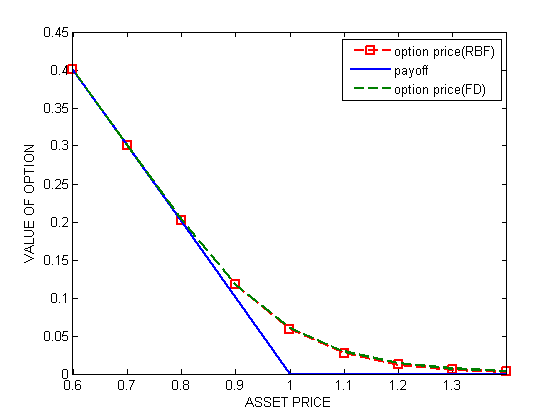
\includegraphics[height=4in]{rbffdpo.png}\
%\caption{Comparison between RBF and Finite Difference Solutions }
%\vskip -0.5in \vskip -0.5in
%\end{centering}
%\end{figure}

\begin{table}[h]
\centering
  \caption{Finite Difference solution at $N=2001,\epsilon=10^{-2},k=0.1$.}\label{Tab_2}
\vspace{5mm}
\begin{tabular}{|c|c|c|c|c|c|c|}
  \hline
  % after \\: \hline or \cline{col1-col2} \cline{col3-col4} ...
  S &  Option Value& FD1001  \\
  \hline

  0.6 & 0.4134769 &0.4000037 \\
  0.7 &0.3191524&0.3001161 \\
  0.8 &0.2295821& 0.2020397 \\
  0.9 & 0.1513232&0.1169591  \\
  1.0 & 0.0913208&0.0602833 \\
  1.1 & 0.0513920&0.0293272\\
  1.2 & 0.0277877&0.0140864 \\
  1.3 & 0.0149302 &0.0038609 \\
  1.4& 0.0082378&0.0038609 \\
 \hline
CPUTIME&0.312002&\\
\hline
 RMSE&0.0216&\\
  \hline

\end{tabular}
  %\caption{Finite Difference solution at $N=2001,\epsilon=10^{-2},k=0.1$.}\label{Tab_2}
\end{table}

\newpage
\begin{figure}
\begin{center}
%\vskip -0.5in
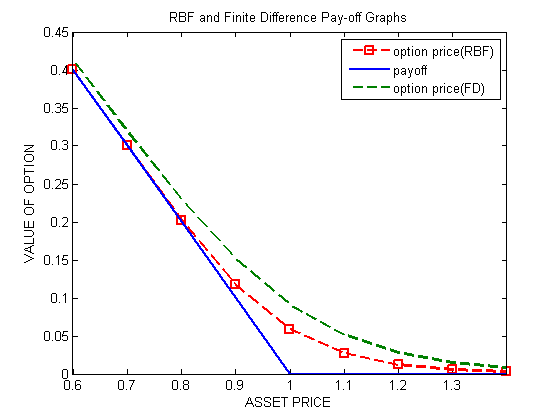
\includegraphics[height=4in]{rbffd101.png}\
\end{center}
\vspace{-0.5in}
 \caption{RBF \textit{N}=101, \textit{k}=0.01 and FD
\textit{N}=2001,\textit{k}=0.01 }
 %\vskip -0.5in
\end{figure}

 \begin{figure}[h]
\begin{center}
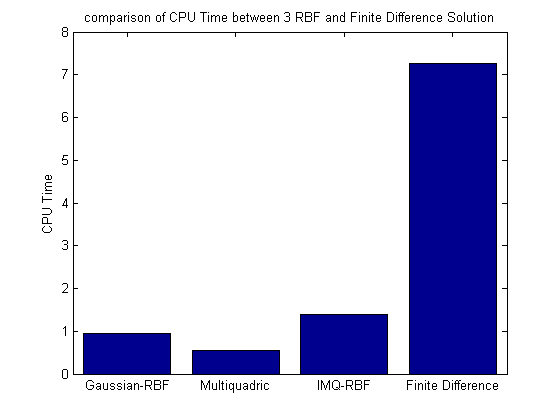
\includegraphics[height=3in]{cpue10000.png}\
\end{center}
\vspace{-0.5in} \caption{Comparison of CPU Times between the 3 RBFs
for $N=101$ and FD for \textit{N}=2001 }
\end{figure}

\begin{figure}[h]
\begin{center}
%\vskip -0.5in
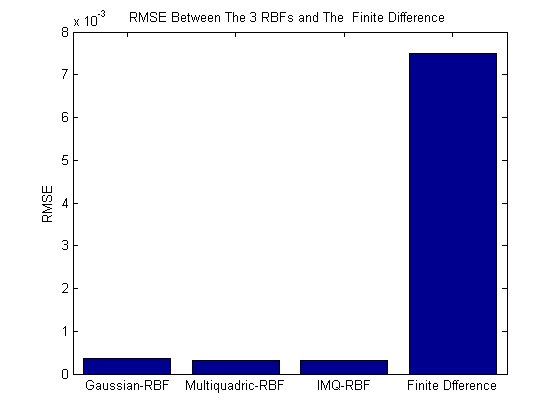
\includegraphics[height=3in]{barrmsee10000.png}\
\end{center}
\vspace{-0.5in} \caption{Comparison of RMSE between the 3 RBFs for
$N=101$ and FD for \textit{N}=2001 }


\end{figure}


%-------------------------------------------------------------------------------------------------------------------------
%================================================ Chapter 8  ==============================================================
\sect{\uppercase{Discussion of Numerical Results  and Conclusion}}

%-------------------------------------------------------------------------------------------------------------------------


\subsection{ Discussion of Numerical Results}

  Meshfree radial basis function
interpolation exercise numerous advantages over traditional finite
difference approximation schemes. RBFs depend on only the scalar
distance between between two nodes at each point,this makes its
discretization to be independent of coordinate system,dimension and
domain geometry. With meshfree methods,it is possible to obtain the
value of the option for different combination of option prices by
evaluating the derivative of the basis function$(\ref{rbf1})$ as
compared to finite difference which requires the inclusion of an
extra interpolation step. RBFS are infinitely differentiable
functions and as such produce highly accurate approximations to
spatial derivatives whereas finite difference approximations  to
spatial derivatives are
mostly second order accurate.\\
   In Table 2,3 and 4,we evaluate  a fair price of the
   American option using Gaussian,Multiquadric and
   Inverse-Multiquadric RBFs at different nodes of 41,81 and 101
   with shape parameter $c=1.5$. It was observed that the level of
   accuracy of the numerical results increased as the number of
   meshpoints was increased. The root mean squared error was
   computed as
   \begin{equation*}
RMSE=\frac{1}{\sqrt{N}}\sqrt{\displaystyle\sum\limits_{i=1}^N
|V(S_j,t)_{RBF}-V(S_j,t)_{FD1001})|^2}
   \end{equation*}
   where $V(S_j,t)_{RBF}$ and $V(S_j,t)_{FD1001})$ are the value of
   the option obtained using RBF meshfree approach  and  the bench
   mark solution in Fasshauer \textit{et al} \cite{Fas02}
   respectively.\\
   The condition number of the matrix $\Phi$ was computed as
   \begin{equation*}
   Condition \hspace{5mm} number(\Phi)=\frac{max \lambda_i}{min \lambda_i}=\|\Phi\|\|\Phi^{-1}\|
   \end{equation*}
   where $\lambda_i$ is an eigenvalue of the matrix $\Phi$.\\
   The choice of an optimal value for the shape parameter $c$ is
  critical to the accuracy and stability of the numerical
  system. There is no precise or definite  approach to choosing an
  optimal value for the shape parameter. Table 5,6 and 7 has several
  values of the shape parameter $c$ with corresponding root mean
  squared error and CPU time at $101$ nodes with parameters  as
  listed in Table 1 for  Gaussian,Multiquadric and
   Inverse-Multiquadric RBFs respectively. Figures $4,5,6,7$ and $8$ are
   based on these values. From figures 4,5 and 6,the optimal value of
   the shape parameter $c$ for Gaussian RBF is $1.5$,$1.0$ for for
   Multiquadric and $1.5$ for Inverse-Multiquadric. The
   Multiquadric -RBF proved to be the most computationally eficient
   and accurate as depicted by figures $7$ and $8$.It has the lowest
   CPU time usage and root mean squared error among the three
   RBFs.\\
   Figure $1,2,3$ represent the values   of a fair price of the American put option obtained
by Gaussian,Multiquadric and Inverse-Multiquadric RBFs at $101$
nodes obtained from Table 1,2,and 3 respectively and their payoff
function with parameters as listed in Table 1.\\
 In Tables $ 8,9$ and $10$,we evaluate the value of the American put
 option by finite difference approximation approach at $2001$
 nodes. It is evident from our numerical results that the accuracy of
 the method greatly improves if the time step $k$ is made smaller
 and smaller. The efficiency of the numerical scheme however
 deteriorates by decreasing the  regularization parameter $\epsilon$.\\
  In figure 9,we compare the value of a fair price of the American
  option by Multiquadric at $101$ nodes to that of finite difference
  approximation at $2001$ nodes.\\
   Figures 10 and 11 confirm that each one of the three RBF meshfree
   approach implemented in our numerical analysis was
   computationally efficient and accurate even at $101$ nodes than a
   finite difference approximation  obtained at $2001$ nodes using
   the solution the solution obtained by Fasshauer \textit{et al}
   \cite{Fas02} as our bench mark solution.


\subsection{Conclusion}
In this thesis,we evaluated a fair price of standard American
options using both radial basis interpolation approach and finite
difference approximation scheme. We implemented numerical solutions
from three different RBFs namely the Gaussisn,Multiquadric and
Inverse-Multiquadric RBFs. The free boundary in the American option
problem was removed by the introduction of a nonlinear continuous
 penalty term. This allowed the problem to be solved on fixed domain.
 The numerical results obtained from our experiments
shows that  the Multiquadric-RBF  is highly efficient and accurate
in computing the value of the  American option. This  confirms its
exponential convergence rate property. Our results suggest that each
of the three RBFs implemented was considerably efficient and
accurate even at a less number of nodes than the finite difference
approximation scheme implemented.

%\numberwithin{equation}{section}
%Meshfree radial basis function interpolation exercise numerous
%advantages over traditional finite difference approximation schemes.
%RBFs depend on only the scalar distance between between two nodes at
%each point,this makes its discretization to be independent of
%coordinate system,dimension and domain geometry.With meshfree
%methods,it is possible to obtain the value of the option for
%different combination of option prices by evaluating the derivative
%of the basis function$(\ref{rbf1})$ as compared to finite difference
%which requires the inclusion of an extra interpolation step.RBFS are
%infinitely differentiable  functions and as such produce highly
%accurate approximations to spatial derivatives whereas finite
%difference approximations  to spatial derivatives are
%mostly second order accurate.\\
%  The choice of an optimal value for the shape parameter $c$ is
%  critical to the accuracy and stability of the numerical
%  system.There is no precise or definite  approach to choosing an
%  optimal value for the shape parameter.In our  numerical
%  simulations,we compared several values of $c$ with their
%  corresponding root mean squared error before arriving at optimal
%  values for each of the RBFs.It was observed that optimal value for
%  Gaussian RBF was $c=1.5$,$c=1.0$ for Multiquadric RBF and $c=1.5$
%  for Inverse-Multiquadric RBF.\\
%    In our study,we compared the RBF approximation approach of
%    evaluating  a fair price of the American put option at$101$
%    nodes to finite difference approximation scheme at $2001$
%    nodes.It was observed that  each of the three RBFs implemented provided
%    much accurate and efficient results than the finite difference
%    scheme using the solution obtained by Fasshauer \textit{et
%    al}(which is based on a very high order finite difference approximation)as our bench mark
%    solution.\\
%    In further research ,we would like to examine each of the three
%    RBFs in terms of accuracy ,computational cost and  efficiency in
%    a two asset American option case.

 %Meshfree radial basis function
%interpolation exercise numerous advantages over traditional finite
%difference approximation schemes. RBFs depend on only the scalar
%distance between between two nodes at each point,this makes its
%discretization to be independent of coordinate system,dimension and
%domain geometry. With meshfree methods,it is possible to obtain the
%value of the option for different combination of option prices by
%evaluating the derivative of the basis function$(\ref{rbf1})$ as
%compared to finite difference which requires the inclusion of an
%extra interpolation step.RBFS are infinitely differentiable
%functions and as such produce highly accurate approximations to
%spatial derivatives whereas finite difference approximations  to
%spatial derivatives are
%mostly second order accurate.\\
%   In Table 2,3 and 4,we evaluate  a fair price of the
%   American option using Gaussian,Multiquadric and
%   Inverse-Multiquadric RBFs at different nodes of 41,81 and 101
%   with shape parameter $c=1.5$. It was observed that the level of
%   accuracy of the numerical results increased as the number of
%   meshpoints was increased. The root mean squared error was
%   computed as
%   \begin{equation*}
%RMSE=\frac{1}{\sqrt{N}}\sqrt{\displaystyle\sum\limits_{i=1}^N
%|V(S_j,t)_{RBF}-V(S_j,t)_{FD1001})|^2}
%   \end{equation*}
%   where $V(S_j,t)_{RBF}$ and $V(S_j,t)_{FD1001})$ are the value of
%   the option obtained using RBF meshfree approach  and  the bench
%   mark solution in Fasshauer \textit{et al} \cite{Fas02}
%   respectively.\\
%   The condition number of the matrix $\Phi$ was computed as
%   \begin{equation*}
%   Condition number(\Phi)=\frac{max \lambda_i}{min \lambda_i}=\|\Phi\|\|\Phi^{-1}\|
%   \end{equation*}
%   where $\lambda_i$ is an eigenvalue of the matrix $\Phi$.\\
%   The choice of an optimal value for the shape parameter $c$ is
%  critical to the accuracy and stability of the numerical
%  system. There is no precise or definite  approach to choosing an
%  optimal value for the shape parameter. Table 5,6 and 7 has several
%  values of the shape parameter $c$ with corresponding root mean
%  squared error and CPU time at $101$ nodes with parameters  as
%  listed in Table 1 for  Gaussian,Multiquadric and
%   Inverse-Multiquadric RBFs respectively.Figures $4,5,6,7$ and $8$ are
%   based on these values.From figures 4,5 and 6,the optimal value of
%   the shape parameter $c$ for Gaussian RBF is $1.5$,$1.0$ for for
%   Multiquadric and $1.5$ for Inverse-Multiquadric. The
%   Multiquadric -RBF proved to be the most computationally eficient
%   and accurate as depicted by figures $7$ and $8$.It has the lowest
%   CPU time usage and root mean squared error among the three
%   RBFs.\\
%   Figure $1,2,3$ represent the values   of a fair price of the American put option obtained
%by Gaussian,Multiquadric and Inverse-Multiquadric RBFs at $101$
%nodes obtained from Table 1,2,and 3 respectively and their payoff
%function with parameters as listed in Table 1.\\
% In Tables $ 8,9$ and $10$,we evaluate the value of the American put
% option by finite difference approximation approach at $2001$
% nodes.It is evident from our numerical results that the accuracy of
% the method greatly improves if the time step $k$ is made smaller
% and smaller.The efficiency of the numerical scheme however
% deteriorates by decreasing the  regularization parameter $\epsilon$.\\
%  In figure 9,we compare the value of a fair price of the American
%  option by Multiquadric at $101$ nodes to that of finite difference
%  approximation at $2001$ nodes.\\
%   Figures 10 and 11 confirm that each one of the three RBF meshfree
%   approach implemented in our numerical analysis was
%   computationally efficient and accurate even at $101$ nodes than a
%   finite difference approximation  obtained at $2001$ nodes using
%   the solution the solution obtained by Fasshauer \textit{et al}
%   \cite{Fas02} as our bench mark solution.
%
%
%


\cleardoublepage

%=================================================BIBLIOGRAPHY==============================================================
\newpage
\begin{center}
{\bf BIBLIOGRAPHY}
\end{center}
\addcontentsline{toc}{section}{\rm BIBLIOGRAPHY \dotfill}
\begin{thebiblio}{99}
%---------------------------------------------------------------------------------------------------------------------------



\bibitem{ADS06}
A.Q.M. Khaliq, D.A. Voss and S.H.K. Kazmi,   \emph{A linearly
implicit predictor-corrector scheme for pricing American options
using a penalty method approach}, Journal of Banking and Finance,30
(2006) 489-502.
\bibitem{KK}
A.Q.M. Khaliq, D.A. Voss and G. E.Fasshauer,\emph{A Parallel Time
Stepping Approach using Mesh-free Approximations for Pricing Options
with Non-Smooth Payouts},The Journal of Risk 10(2009) 135-142.

\bibitem{BEN11}
B. Fornberg, E. Larsson, and N. Flyer,\emph{ Stable computations
with Gaussian Radial Basis Functions}, SIAM Journal on Scientific
Computing, 33 (2011), 869-892.

\bibitem{BSA02}
B. Nielsen, O. Skavhaug, and A. Tveito, \emph{Penalty and
front-fixing methods for the numerical solution of American option
problems}, Journal of Computational Finance, 5 (2002) 69-97.
\bibitem{BOA08}
B. Nielsen, O. Skavhaug, and A. Tveito,\emph{ Penalty methods for
the numerical solution of American multi-asset option problems},
Journal of Computational and Applied Mathematics, 222 (2008) 3-16.
\bibitem{higham}
D. J. Higham , \emph{An Introduction to Financial Option
Valuation},Cambridge Univeristy Press(2004).
\bibitem{BS73}
F. Black and M.S. Scholes, \emph{The pricing of options and
corporate liabilities}, Journal of Political Economy 81 (1973)
637-659.
\bibitem{Fas02}
G.E. Fasshauer, A.Q.M. Khaliq and D.A. Voss, \emph{Using meshfree
approximation for multi-asset American option problems}, Journal of
Chinese Institute of Engineers, 27 (2004) 563-571

\bibitem{NB11}
N. Flyer and B. Fornberg,\emph{ Radial basis function: Development
and applications to planetary scale flows, Computers and Fluids}
46(2011) 23-32.
\bibitem{Wilmot}
P. Wilmot,S. Howson and J. Dewynne,\emph{The Mathematics of
Financial Derivatives}:A Student Introduction.Cambridge University
Press(1995).
\bibitem{SE09}
S. A. Sarra and E. J. Kansa,  \emph{Multiquadric Radial Basis
Function Approximation Methods for the Numerical Solution of Partial
Differential Equations}. Advances in Computational Mechanics, Tech
Series Press, 2 (2009).
\bibitem{Hon}
Y.C. Hon and X.Z. Mao,\emph{A Radial Basis Function Method for
    Solving Options Pricing Models}.The Journal of Financial
    Engineering,8(1999) 31-49.
\bibitem{YZE07}
Y. Goto, Z. Fei, S.Kan, and E. Kita, \emph{Options valuation by
using radial basis function approximation}, Engineering Analysis
with Boundary Elements, 31(2007) 836-843.
\bibitem{Hon09}
Y.C. Hon and Z. Yang, \emph{Meshless collocation method by
Delta-shaped basis functions for default barrier model}, Engineering
Analysis with Boundary Elements 33(2009) 951-958.


\bibitem{UEG}
U.  Pettersson, E. Larsson, G.  Marcusson, and J. Persson,
\emph{Improved radial basis function methods for multi-dimensional
option pricing}, Journal of Computational and Applied Mathematics,
222 (2008) 82-93.

%\bibitem{PSJ}
%Paul Wilmott,Sam Howson,Jeff Dewynne  \emph{The Mathematics of
%Financial Derivatives}. A Student Introduction, Cambridge university
%press.

%\bibitem{CF}
%Omur Ogur \emph{An Introduction to Computational Finance}.Imperial
%College press




%\bibitem{GEF}
%G.E. Fasshauer,\emph{Meshfree Methods}.Handbook of Theoretical and
%Computational Nanotechnology,M.Rieth and W.Schommers(eds.).American
%Scientific Publishers .(2006)
\end{thebiblio}
\newpage
%=================================Appendix separation page ===========================================================
\Appendixpage
%---------------------------------------------------------------------------------------------------------------------

%%================================================= Appendix A =========================================================
%\appen{\uppercase{ Sample Appendix}}\label{app1}
%%-------------------------------------------------------------------------------------------------------------------






%=========================Appendix ===================================================================================
\appen{\uppercase{Computer Programming Codes}}\label{app2}
%----------------------------------------------------------------------------------------------------------------------

%\subsection{Computer Programming Codes}
\subsubsection{Exact Conditional Test Application with Edge Data}
%\lstinputlisting{tridiagonal.m}

%\lstinputlisting{RBasis3GaussianG.m}
%\lstinputlisting{RBasis3GaussianMQ.m}
%\lstinputlisting{RBasis3GaussianIMQ.m}
%\lstinputlisting{tridiagonal.m}
\lstinputlisting{Edge.R}

\subsubsection{Stratified Linear Exact Test}

\lstinputlisting{wilcoxon.R}

\lstinputlisting{stratified.R}


%\begin{verbatim}
%function y=lbc(E,T,r,t)
%% Boundary Condition at s=0;
%%Black-Scholes Equation
%%E=1;r=0.1;
%%T=1;
%%***********************************
%% PUT
%% y=E*exp(-r*(T-t));
%%y=E;
%%*************************************
%% CALL
%y=0;
%\end{verbatim}


\end{document}
